\documentclass[aspectratio=169]{beamer}

\usepackage[utf8]{inputenc}
\usepackage{times}
\usepackage{mathptmx}

\usepackage{graphicx}
\usepackage[outdir=./figs/]{epstopdf}
\graphicspath{ {./figs/} }

\usepackage{amsmath} % función de corte


%%%%% definición de colores para el tema
\usetheme{Madrid}
\useoutertheme{infolines} % Alternatively: miniframes, infolines, split
\useinnertheme{circles}

\definecolor{nordwhite}{rgb}{0.9255, 0.9373, 0.9569}
\definecolor{nordgrey}{rgb}{0.298, 0.3373, 0.4157}
\definecolor{nordblue}{rgb}{0.3686, 0.5059, 0.6745} % nord blue (primary)
\definecolor{nordlblue}{rgb}{0.5059, 0.6314, 0.7569}
\definecolor{nordllblue}{rgb}{0.5333, 0.752, 0.8157} % nord lblue (secondary)
\definecolor{nordlllblue}{rgb}{0.5608, 0.7373, 0.7333}

\setbeamercolor{background canvas}{bg=nordwhite}
\setbeamercolor{normal text}{fg=nordgrey}

\setbeamercolor{palette primary}{bg=nordblue,fg=nordwhite}
\setbeamercolor{palette secondary}{bg=nordlblue,fg=nordwhite}
\setbeamercolor{palette tertiary}{bg=nordllblue,fg=nordwhite}
\setbeamercolor{palette quaternary}{bg=nordlllblue,fg=nordwhite}

\setbeamercolor{structure}{fg=nordblue} % itemize, enumerate, etc
\setbeamercolor{section in toc}{fg=nordblue} % TOC sections

% Override palette coloring with secondary
\setbeamercolor{subsection in head/foot}{bg=nordlblue,fg=nordwhite}

% textbf con otro color
\let\oldtextbf\textbf
\renewcommand{\textbf}[1]{\textcolor{nordblue}{\oldtextbf{#1}}}

%%%%% caratula
\title[Potenciales de ML]{Potenciales interatómicos de aprendizaje automático y 
su aplicación a baterías de litio}
\subtitle{Seminario de doctorado}
\author[Francisco FERNANDEZ]{Francisco FERNANDEZ}
\logo{
    
\includegraphics[width=1.3cm,keepaspectratio]{logo_famaf.png}
}
\institute[FaMAF - UNC]{Facultad de Matemática, Astronomía, Física y Computación 
(Universidad Nacional de Córdoba) \\ \scalebox{1.5}{\insertlogo}}
\date[\today]{\today}

% tabla de contenidos
\AtBeginSection[]
{
	\begin{frame}
		\frametitle{Índice}
		\tableofcontents[currentsection]
	\end{frame}
}

\begin{document}

    \frame{\titlepage}
	
	\begin{frame}
        \frametitle{Índice}
		\tableofcontents
	\end{frame}

    %%%% INTRODUCCION %%%%
    \section{Introducción}
    
    \begin{frame}
        \frametitle{Introducción: Funcionamiento de una batería}

        \begin{columns}
            \column{0.5\textwidth}
            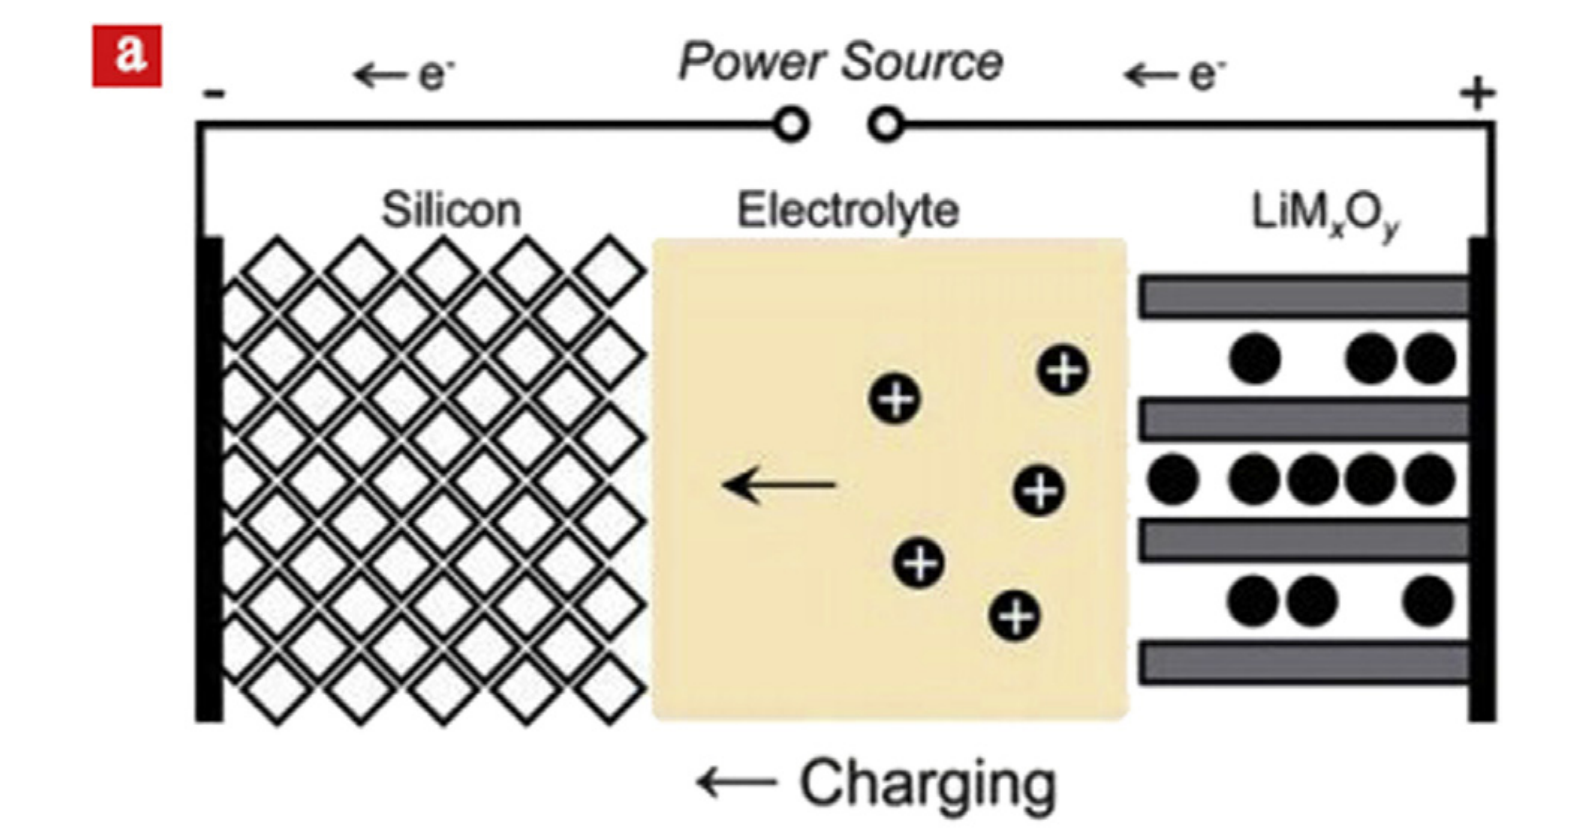
\includegraphics[width=\columnwidth]{intro-bateria-carga.png}
            \pause
            \column{0.5\textwidth}
            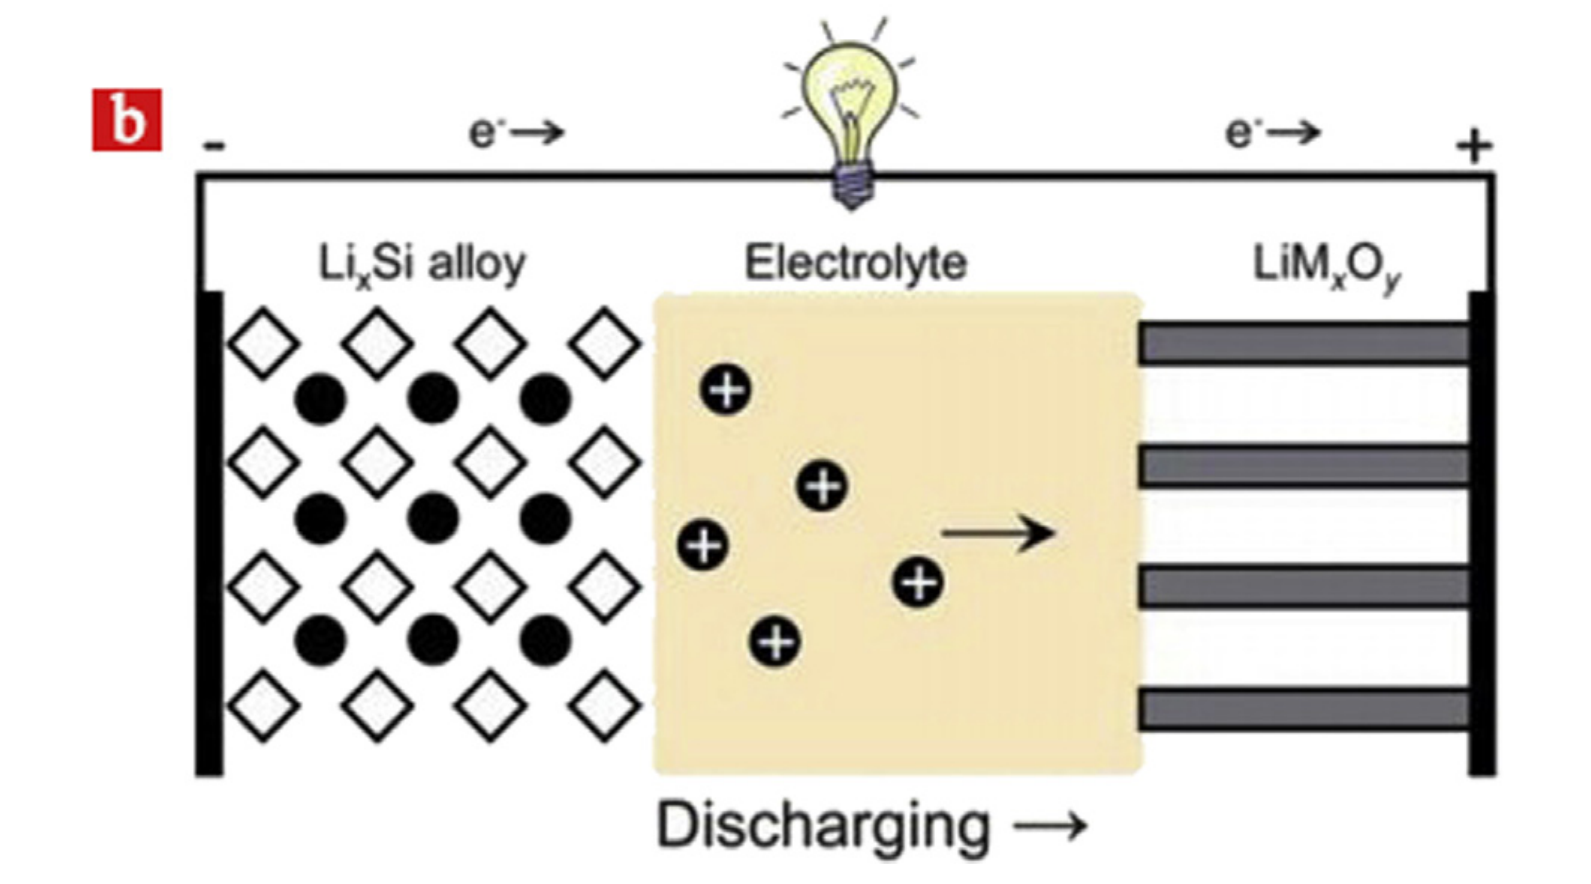
\includegraphics[width=\columnwidth]{intro-bateria-descarga.png}
        \end{columns}

	\end{frame}
    
    \begin{frame}
        \frametitle{Introducción}
        
        Para complementar la gran cantidad de \textbf{herramientas experimentales}
        (difracción de rayos x o neutrones, microscopía electrónica, resonancia
        magnética nuclear, espectroscopía de rayos x, etc) que existen para 
        estudiar materiales relevantes para las distintas partes de las baterías 
        se han venido realizando \textbf{simulaciones computacionales}, 
        principalmente:
        \begin{enumerate}
            \item Teoría del funcional de la densidad electrónica (DFT),
            \item campos de fuerzas (FF) en MD, MC, kMC, etc.
        \end{enumerate}

        \ \pause

        En este seminario se presenta un modelado emergente y complementario, los
        \textbf{potenciales interatómicos de aprendizaje automático} entrenados a 
        partir de datos de referencia provenientes de mecánica cuántica que buscan
        tener eficiencia y precisión cercanas a las de los FF y de DFT, 
        respectivamente.

	\end{frame}

    \begin{frame}
        \frametitle{Introducción}

        En la aproximación de Born-Oppenheimer, donde los núcleos de los átomos
        son considerados como partículas clásicas a la hora de determinar la 
        función de onda electrónica, la energía de un estado electrónico a partir 
        de las posiciones de los núcleos se conoce como la \textbf{superficie 
        energía-potencial (PES)} y está completamente definida por su Hamiltoniano
        electrónico.

        \pause

        \begin{center}
            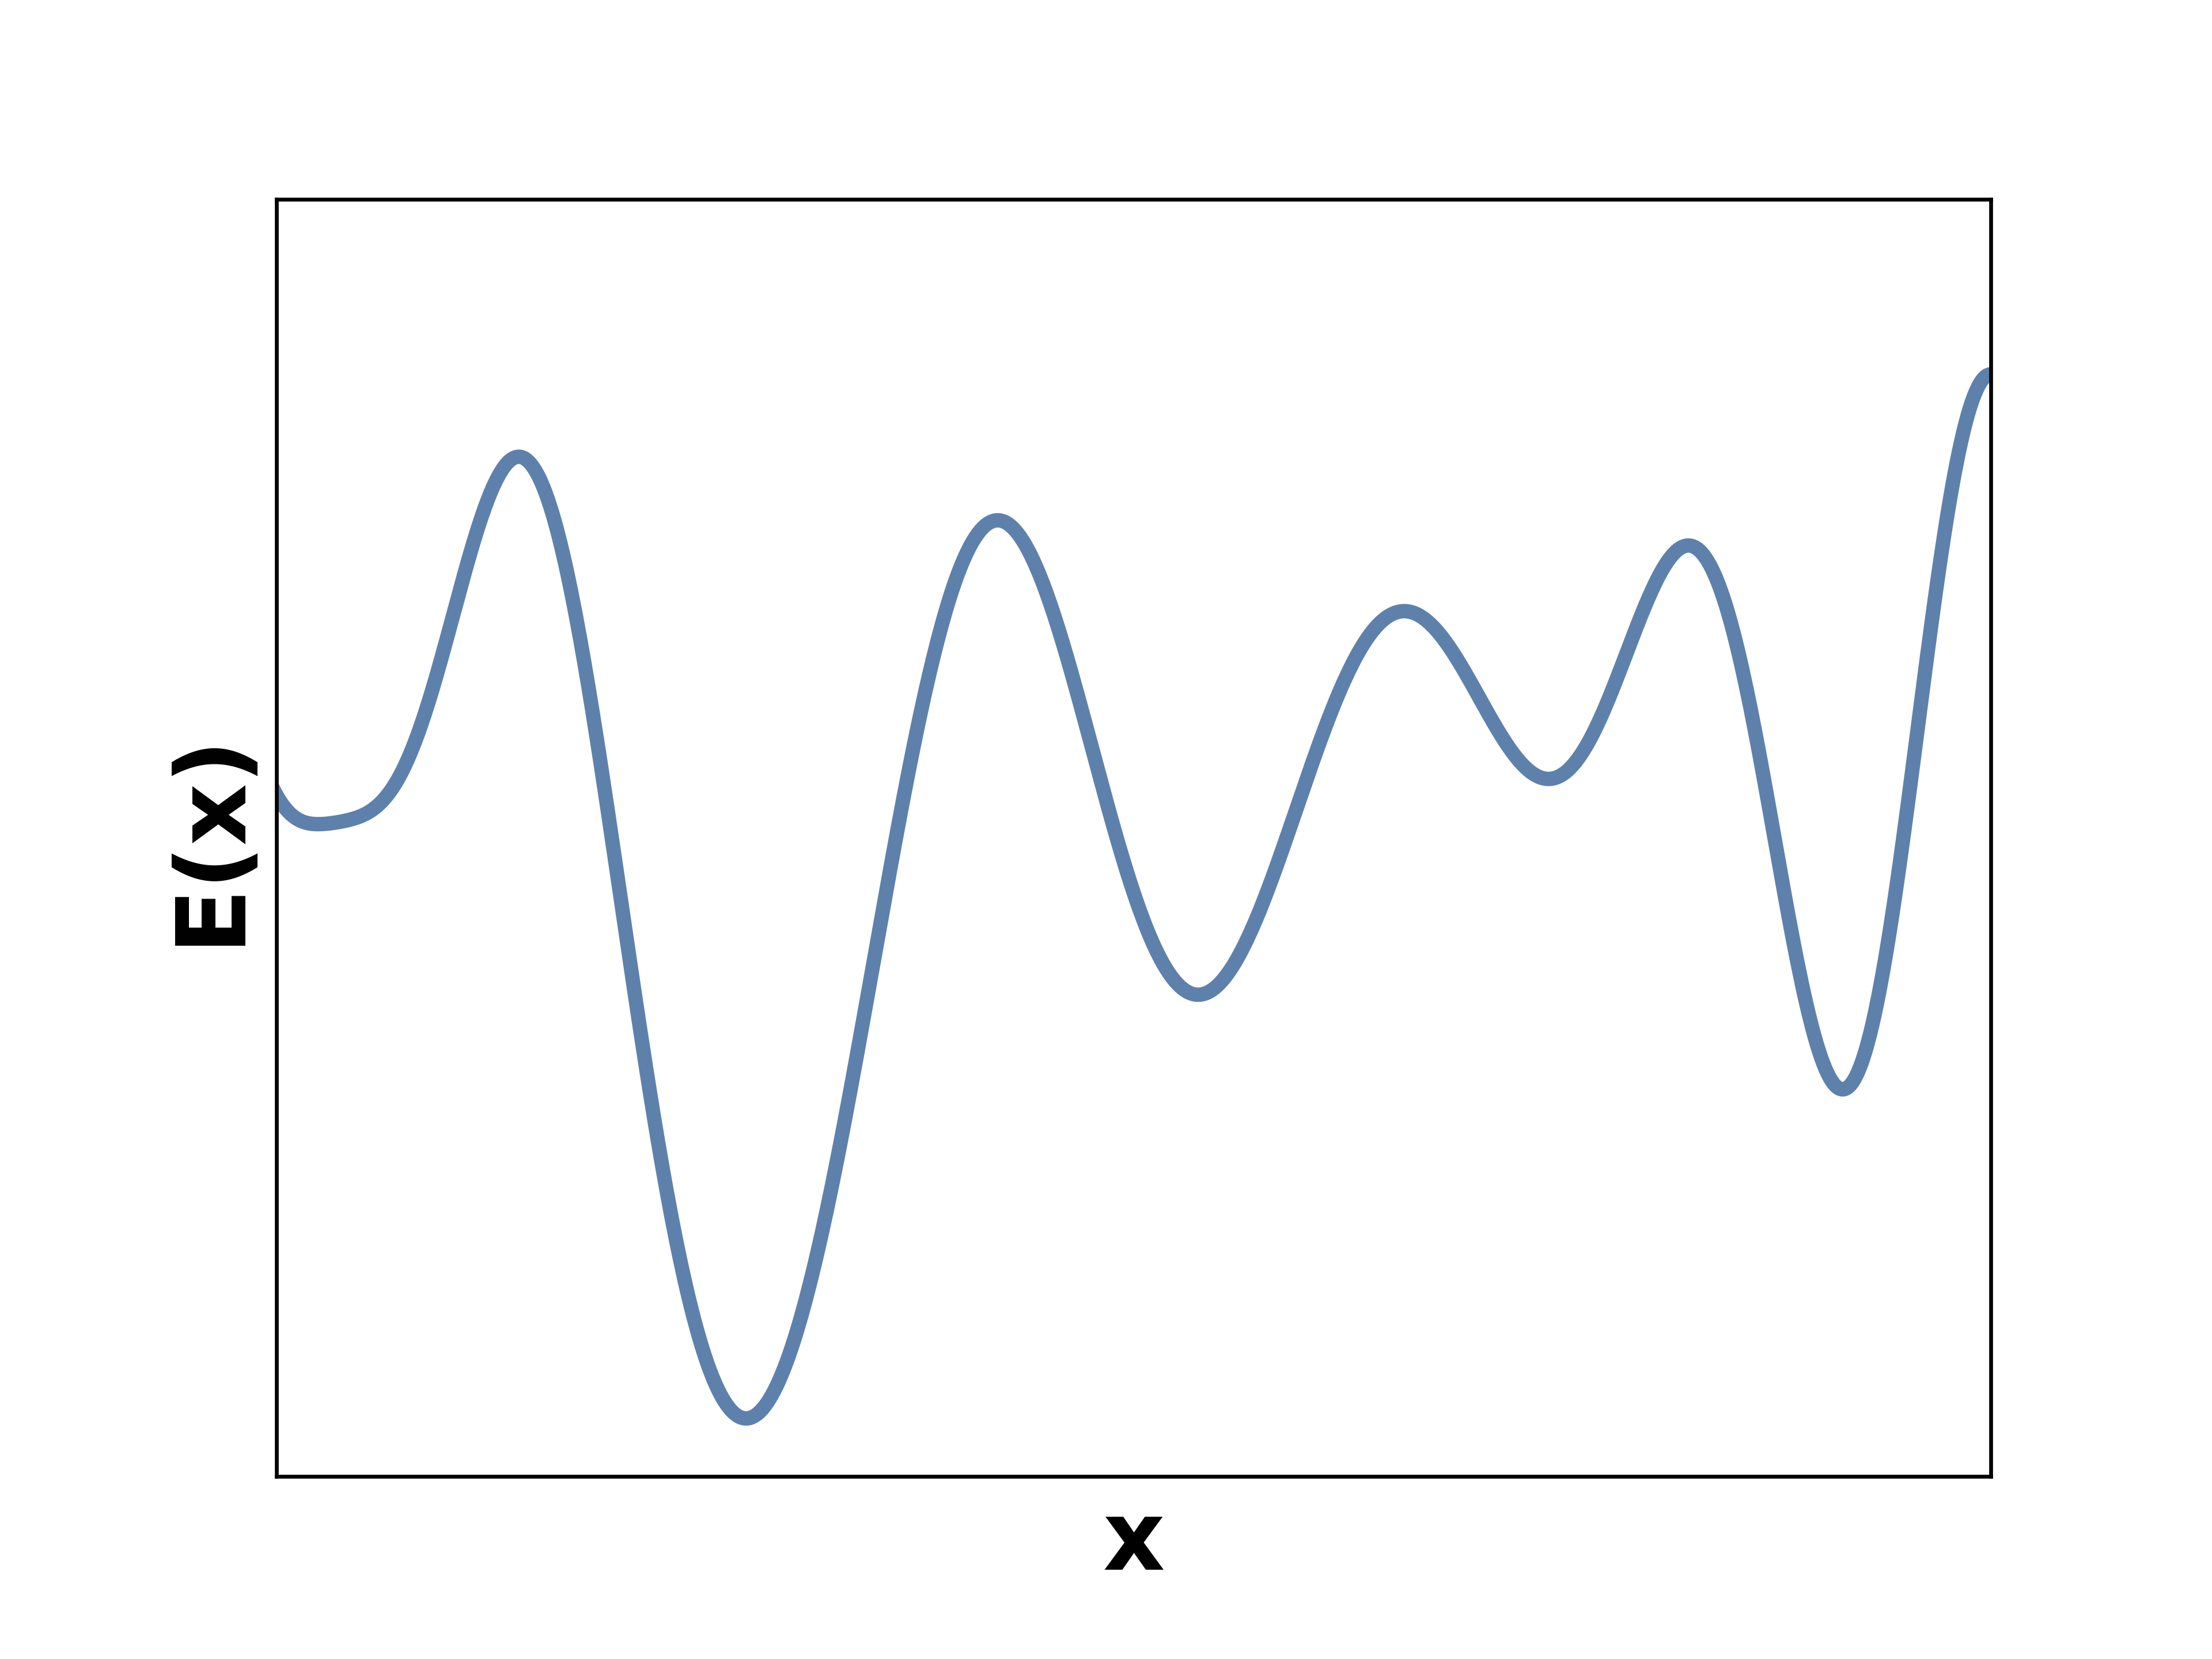
\includegraphics[width=0.35\textwidth]{intro-pes.png}
        \end{center}

	\end{frame}

    \subsection{Teoría del Funcional de la Densidad electrónica (DFT)}

	\begin{frame}
        \frametitle{Introducción: Teoría del Funcional de la Densiadad (DFT)}
        
        La forma más precisa de obtener distintos puntos de la \textbf{PES} 
        es a partir de cálculos de mecánica cuántica. Para estados estacionarios 
        tenemos que la ecuación de Schrödinger es 
        $$
        \hat{H} |\psi\rangle = E |\psi\rangle
        $$
        %$$
        %\hat{H} |\psi_n(t)\rangle = i\hbar\frac{\partial}{\partial t} |\psi_n(t)\rangle
        %$$
        \pause

        Para aproximar la solución a esta ecuación, uno de los métodos más 
        utilizados es la \textbf{Teoría del Funcional de la Densidad electrónica 
        (DFT)}.

        \pause

        \begin{columns}
            \column{0.5\textwidth}
            \begin{itemize}
                \item Preciso.
            \end{itemize}

            \column{0.5\textwidth}
            \begin{itemize}
                \item Algunos cientos de átomos y tiempos menores al ns.
                \item Escalea al cubo de la cantidad de electrones.
            \end{itemize}
        \end{columns}
        
	\end{frame}
    
    \subsection{Potenciales interatómicos empíricos (FF)}
	
    \begin{frame}
        \frametitle{Introducción: Potenciales interatómicos empíricos (FF)}

        Una aproximación a la \textbf{PES} puede obtenerse a partir de potenciales
        interatómicos o campos de fuerza (\textit{force fields}, \textbf{FF}), que
        relacionan directamente, a través de una forma funcional, la configuración
        atómica con la energía:
        
        \pause

        \begin{columns}
            \column{0.5\textwidth}
            \begin{itemize}
                \item potencial de Coulomb,
                \item potencial de Lennard-Jones,
                \item método del átomo embebido (EAM),
                \item ReaxFF.
            \end{itemize}
            \column{0.5\textwidth}
            \begin{center}
                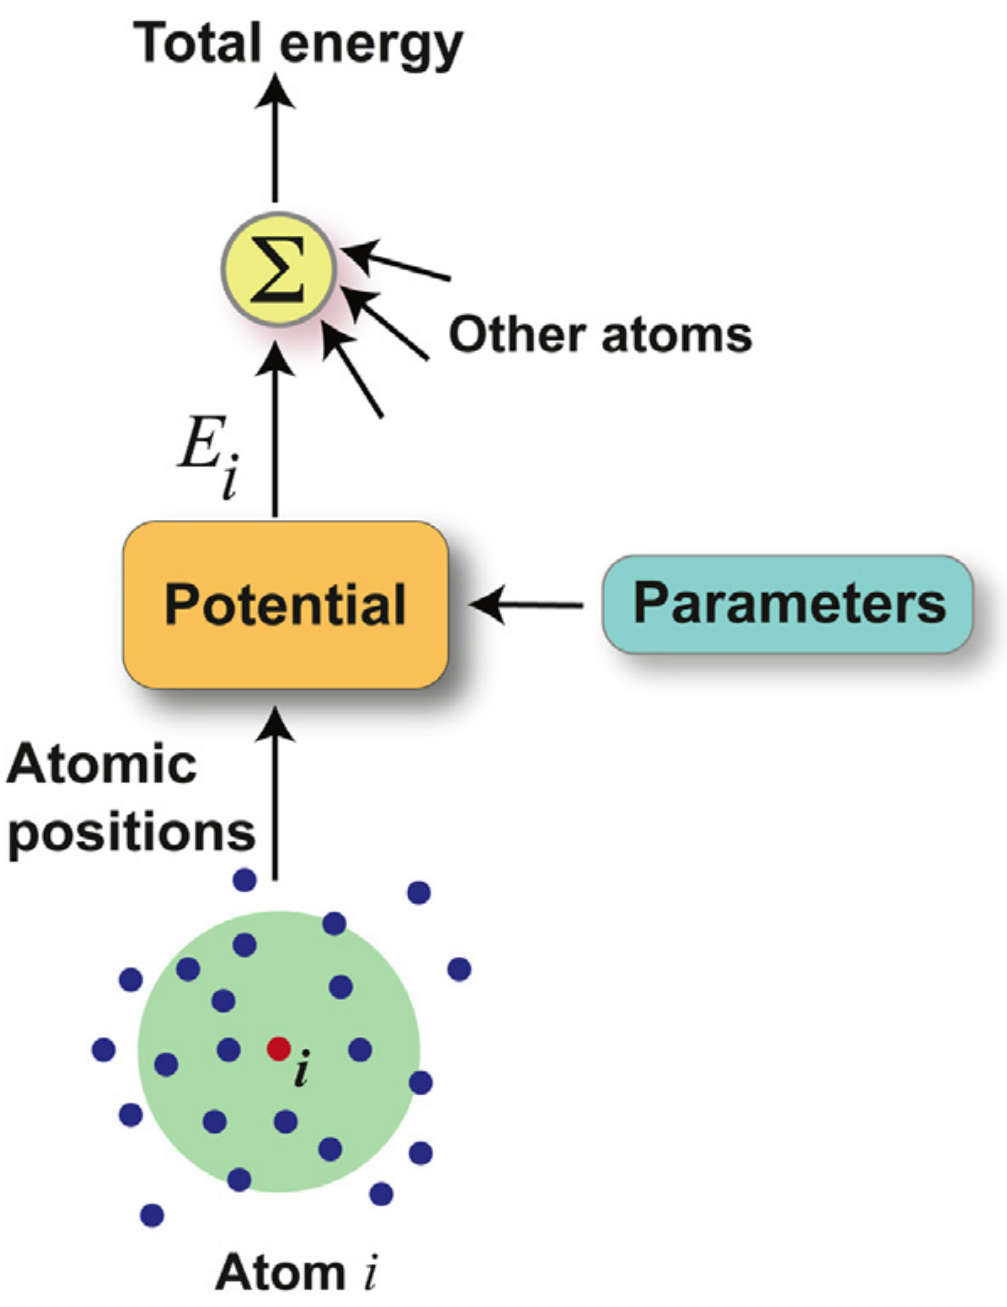
\includegraphics[width=0.4\columnwidth]{intro-ff.png}
        
                \tiny{Mishin (2021). \textit{Acta Materialia}}
            \end{center}
        \end{columns}

        \pause
        
        \begin{columns}
            \column{0.5\textwidth}
            \begin{itemize}
                \item Escalas de tiempo y tamaños más grandes que DFT.
            \end{itemize}

            \column{0.5\textwidth}
            \begin{itemize}
                \item Precisión limitada por la forma funcional.
            \end{itemize}
        \end{columns}

	\end{frame}
    
    \subsection{Potenciales interatómicos de aprendizaje automático (ML)}
    
    \begin{frame}
        \frametitle{Introducción: Potenciales interatómicos de aprendizaje 
        automático (ML)}

        %\begin{center}
        %    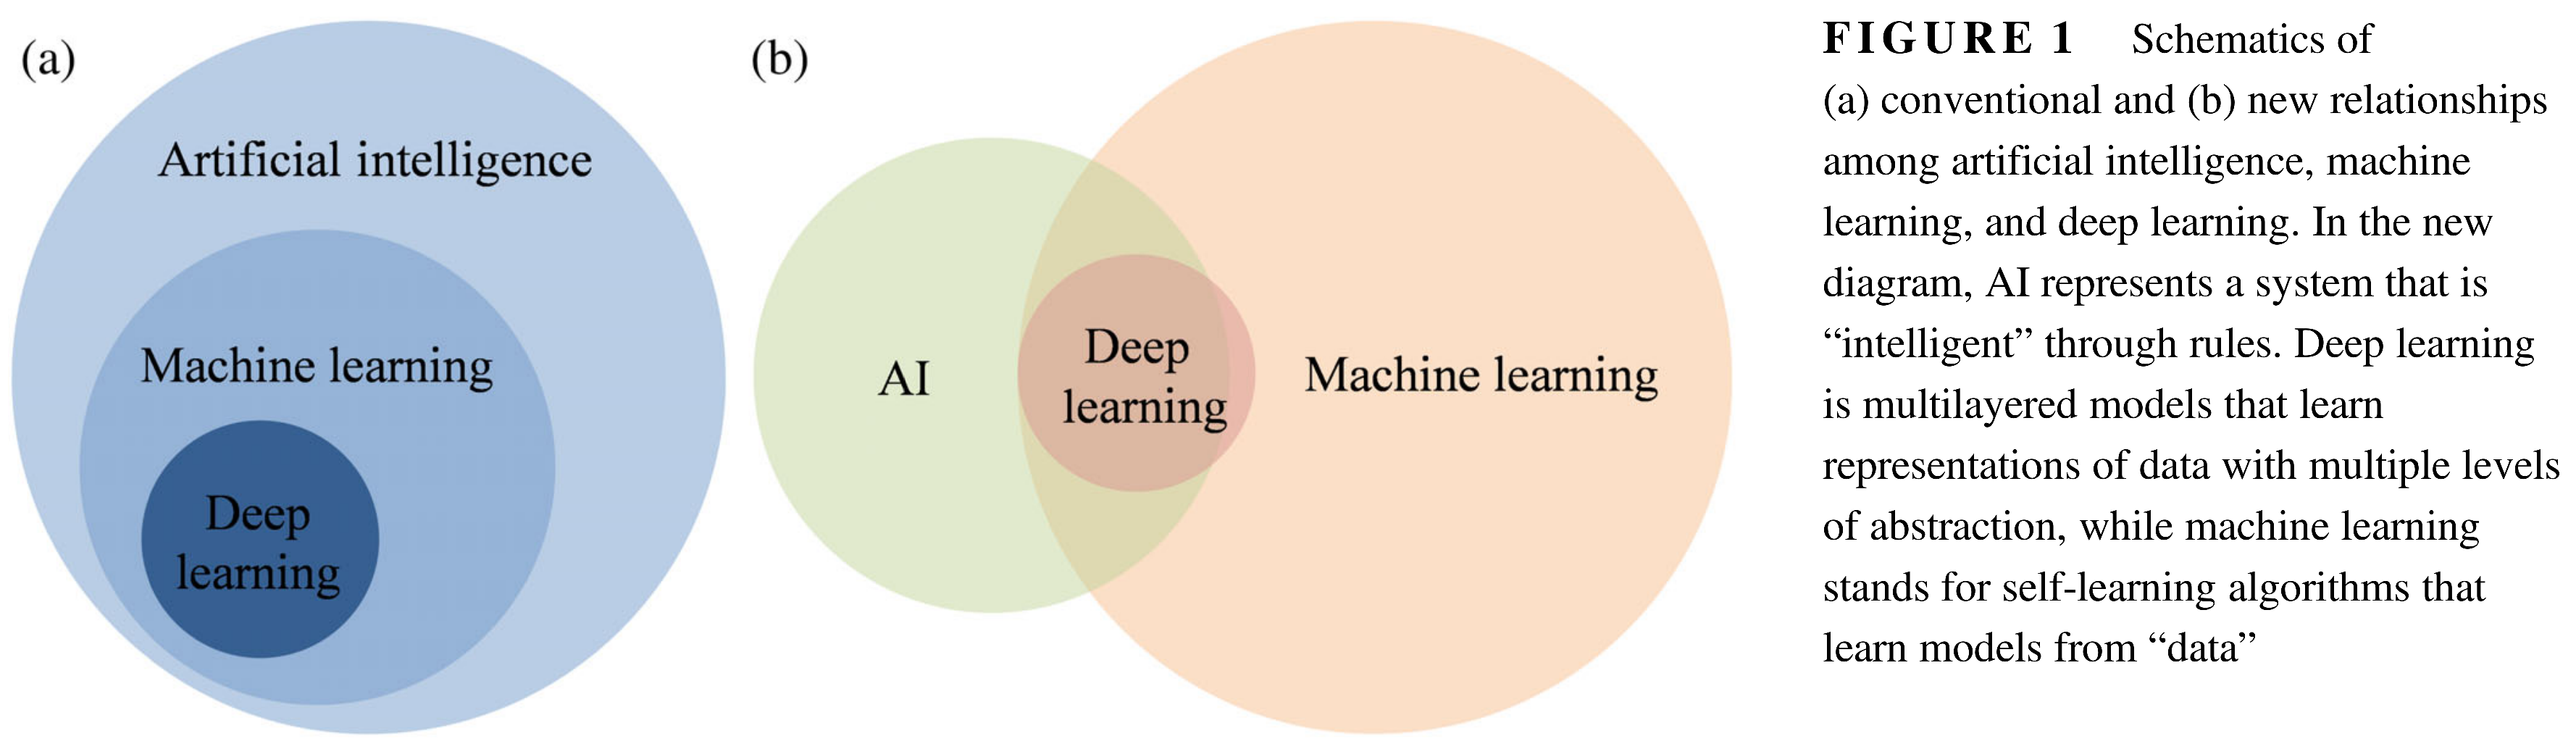
\includegraphics[width=0.7\textwidth]{intro-definicion-ML.png}
        %
        %    \tiny{Hong \textit{et al.} (2020). \textit{Wiley Interdisciplinary
        %    Reviews: Computational Molecular Science}}
        %\end{center}

        El \textbf{aprendizaje automático} puede aprender alguna relación entre 
        datos y etiquetas, si se cuenta con una gran cantidad datos.

        \ \pause
    
        En física, química, ciencias de los materiales, los métodos de aprendizaje
        automático se utilizan para buscar en grandes bases de datos relaciones 
        ocultas entre la \textbf{estructura atómica} y alguna \textbf{propiedad}
        de interés.

        \ \pause

        El tema de este seminario es la aplicación de algunos de estos métodos
        para ajustar la PES en función del entorno atómico.

	\end{frame}
	
    \begin{frame}
        \frametitle{Introducción: Potenciales interatómicos de aprendizaje 
        automático (ML)}

        En el aprendizaje automático supervisado el objetivo es identificar una
        función $f$ (\textit{potencial interatómico que se desea aprender}) que
        prediga valores $y$ (\textit{PES}) a partir de datos de entrada $x$ 
        (\textit{configuraciones de los átomos}).
        
        $$
        y = f(x)
        $$

        \ \pause
        
        Los \textbf{potenciales interatómicos de aprendizaje automático (MLP)} 
        buscan combinar ambas ventajas de los FF (eficiencia) y de DFT 
        (precisión).

	\end{frame}
    
    \begin{frame}
        \frametitle{Introducción: Potenciales interatómicos de aprendizaje 
        automático (ML)}

        Los MLP pueden definirse de la siguiente manera:
        \begin{itemize}
            \item Utiliza un método de ML para construir una relación funcional
                entre las configuraciones atómicas y su energía,
            \item no contienen aproximaciones físicas, a parte del método 
                utilizado para obtener los datos de referencia,
            \item se desarrolla utilizando un conjunto coherente de datos de
                estructura electrónica.
        \end{itemize}

    \end{frame}

    %%%% POTENCIALES INTERATÓMICOS DE APRENDIZAJE AUTOMÁTICO %%%%
    \section{Potenciales interatómicos de aprendizaje automático}

    \subsection{Construcción}

    \begin{frame}
        \frametitle{Potenciales interatómicos de aprendizaje automático: Construcción}

        Pasos en la construcción de un MLP:
        \begin{enumerate}
            \item Cálculos de la estructura electrónica,
            \item preparación de los datos,
            \item construcción de la PES,
            \item validación y
            \item aplicación en simulaciones.
        \end{enumerate}

        \begin{center}
            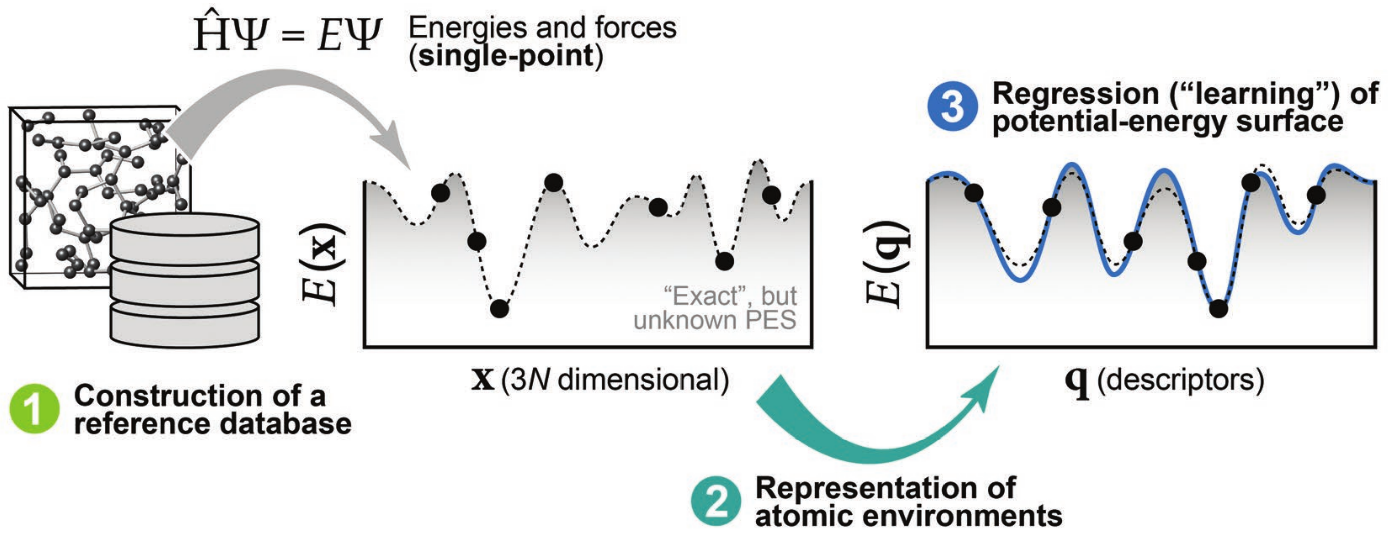
\includegraphics[width=0.65\textwidth]{intro-construccion.png}

            \tiny{Deringer \textit{et al.} (2019). \textit{Advanced Materials}}
        \end{center}

	\end{frame}
    
    \begin{frame}
        \frametitle{Potenciales interatómicos de aprendizaje automático: Construcción}
        
        \begin{columns}
            \column{0.45\textwidth}
            \textbf{1. Cálculos de la estructura electrónica}: Las estructuras deben
            ser elegidas con cuidado para asegurarse que en la PES se encuentren 
            todas las propiedades de interés

            \column{0.55\textwidth}
            \begin{center}
                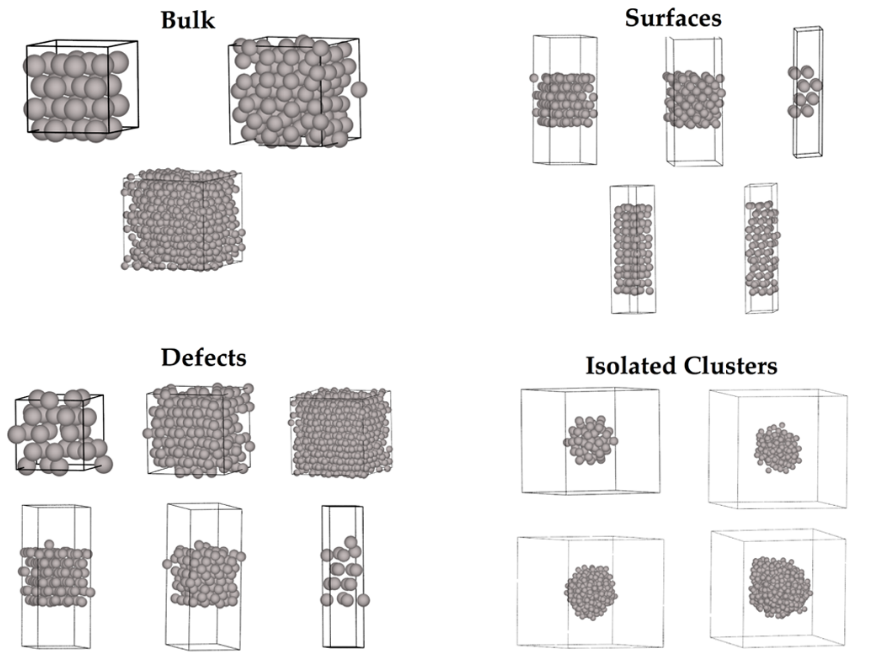
\includegraphics[width=\columnwidth]{intro-dft_data.png}

                \tiny{Botu \textit{et al.} (2016). \textit{The Jornal of Physical
                Chemistry C}}
            \end{center}
        \end{columns}

    \end{frame}
    
    \begin{frame}
        \frametitle{Potenciales interatómicos de aprendizaje automático: Construcción}

        \textbf{2. Preparación de los datos}: Las posiciones atómicas necesitan 
        ser transformadas a \textbf{descriptores} adecuados para los 
        \textbf{métodos de ML} que deben cumplir con distintos \textit{constrains} 
        físicos:
        \begin{enumerate}
            \item Las contribuciones dominantes a la energía son de los átomos 
                más cercanos entre sí.
            \item La energía es invariante a permutaciones entre átomos del mismo 
                tipo, rotaciones, traslaciones.
            \item La PES varía suavemente con respecto a variaciones de las
                posiciones atómicas.
        \end{enumerate}

	\end{frame}
    
    \begin{frame}
        \frametitle{Potenciales interatómicos de aprendizaje automático: Construcción}

        \begin{columns}
            \column{0.35\textwidth}
            \begin{center}
                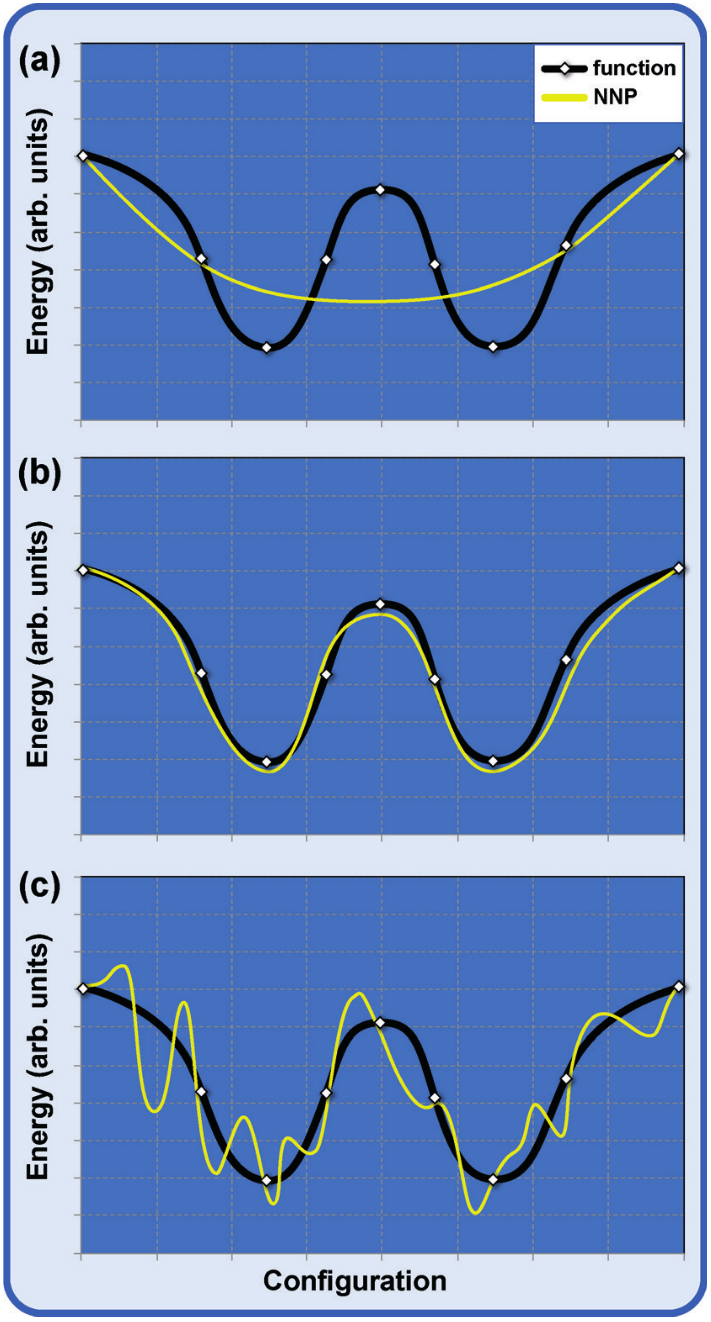
\includegraphics[width=0.65\columnwidth]{intro-fitting.png}
                
                \tiny{Behler (2017). \textit{Angewandte Chemie International}}
            \end{center}

            \column{0.65\textwidth}
            \textbf{3. Construcción de la PES}: Elección del método de ML y 
            proceso de ajuste de los parámetros para que minimicen, usualmente, 
            el RMSE de las energías y de las fuerzas en el conjunto de 
            entrenamiento.

            \

            \textit{underfitting, reasonable fit \& overfitting}.
        \end{columns}

	\end{frame}
    
    \begin{frame}
        \frametitle{Potenciales interatómicos de aprendizaje automático: Construcción}

        \textbf{4. Validación}:
        \begin{enumerate}
            \item \textit{split}: conjunto de entrenamiento / conjunto de testeo.
            \item Se debe ir chequeando si las estructuras de interés están dentro
                del rango de los descriptores usados en el conjunto de 
                entrenamiento
            \item Identificar regiones de la PES insuficientemente muestreadas 
                (por ejemplo, comparando resultados de entrenamientos distintos).
        \end{enumerate}

	\end{frame}

    \begin{frame}
        \frametitle{Potenciales interatómicos de aprendizaje automático: Construcción}
        
        \textbf{5. Aplicación en simulaciones}:

        \begin{columns}
            \column{0.5\textwidth}
            \begin{center}
                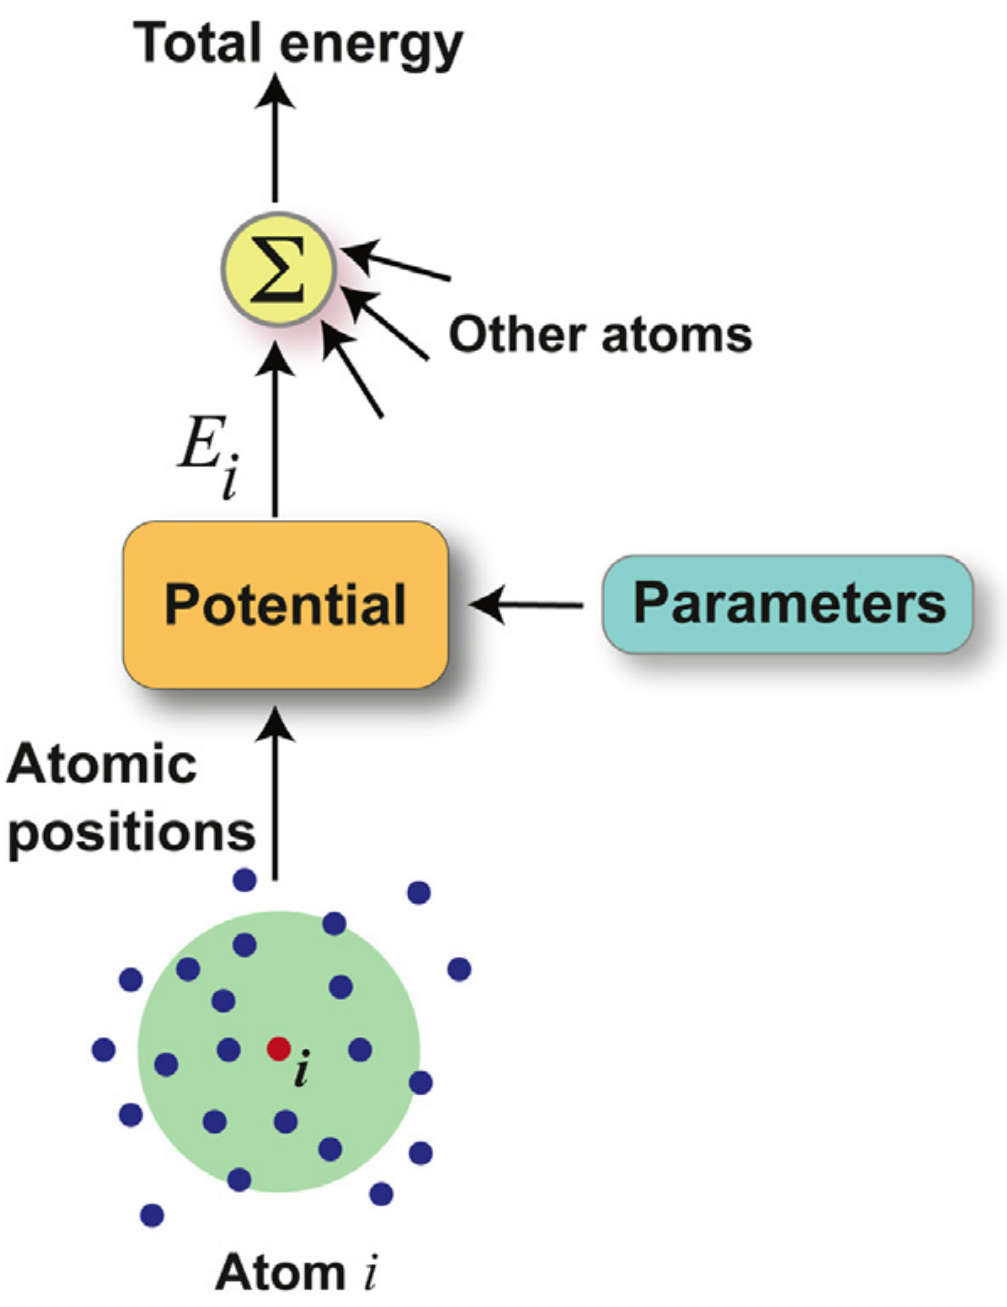
\includegraphics[width=0.5\columnwidth]{intro-ff.png}
            \end{center}
            \column{0.5\textwidth}
            \begin{center}
                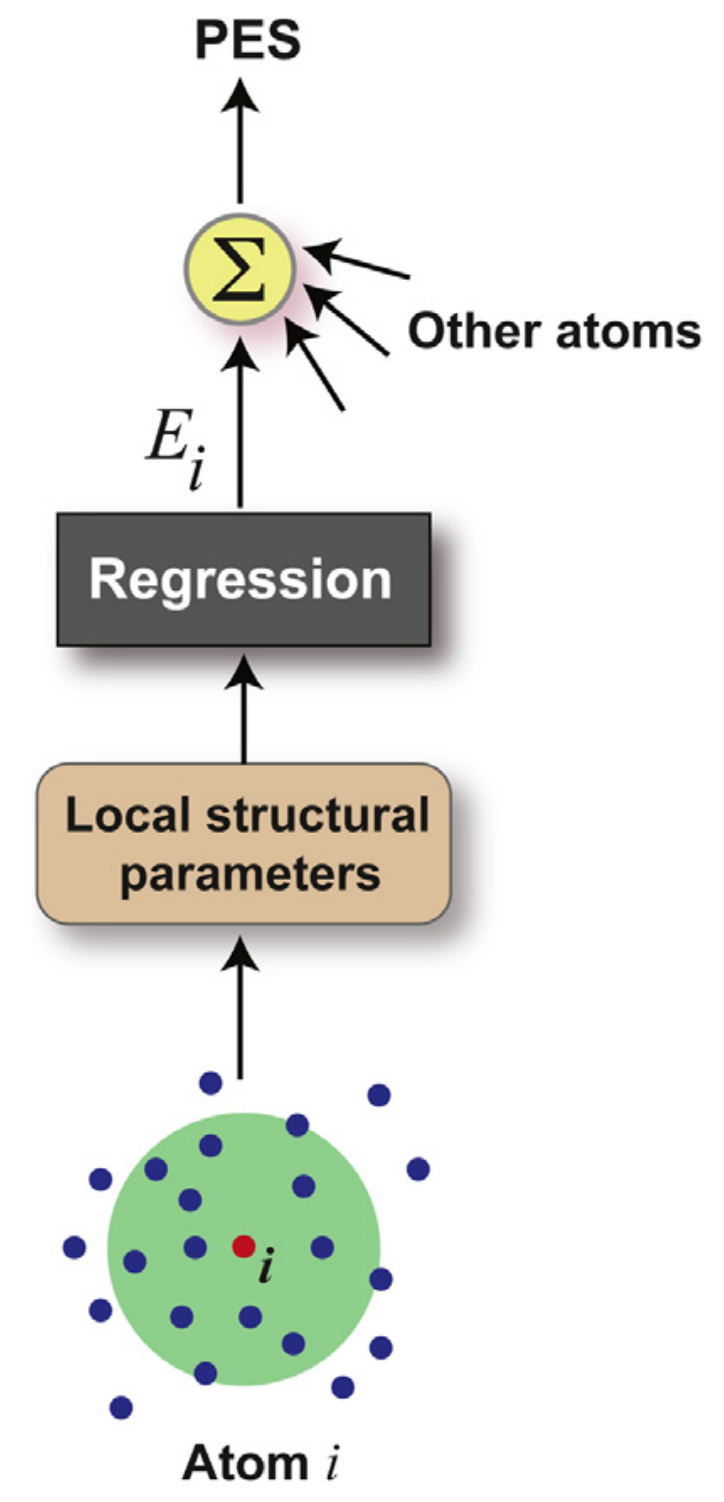
\includegraphics[width=0.3\columnwidth]{intro-ml.png}
            \end{center}
        \end{columns}

        \tiny{Mishin (2021). \textit{Acta Materialia}}

	\end{frame}

    \subsection{Descriptores}
    \begin{frame}
        \frametitle{Potenciales interatómicos de aprendizaje automático: Descriptores}
        
        \begin{itemize}
            \item Se tiene que obtener el mismo output si las estructuras son 
                equivalentes (en los potenciales clásicos viene dado por la 
                expresión matemática).
            \item Correspondencia 1 a 1 entre estructura y los valores del 
                descriptor.
            \item Deben ser rápidos de calcular y diferenciables con respecto a 
                las posiciones atómicas.
        \end{itemize}

    \end{frame}

    \begin{frame}
        \frametitle{Potenciales interatómicos de aprendizaje automático: Descriptores}

        \textbf{Funciones de simetría centradas en el átomo (ACSF)}: El entorno
        químico está caracterizado por descriptores que dependen de las posiciones
        de los átomos hasta un radio de corte $R_c$


        \[ f_c(R_{ij}) = 
            \begin{cases}
                \frac{1}{2}\left( \cos\left(\frac{\pi R_{ij}}{R_c}\right) + 1 \right) & R_{ij} \leq R_c \\
                0 & R_{ij} > R_c
            \end{cases}
        \]
        
        \pause

        \textbf{Función radial}:
        $$
        G_i^{atom,rad} = \sum_{j=1}^{N_{atom}} e^{- \eta (R_{ij} - R_s)^2} \cdot f_c(R_{ij})
        $$

        \textbf{Función angular}
        $$
        G_i^{atom,rad} = 2^{1-\xi}  \sum_{j,k \neq i}^{all} (1 + \lambda \cos(\theta_{ijk}))^{\xi} e^{- \eta (R_{ij}^2 + R_{ik}^2 + R_{jk}^2)} \cdot f_c(R_{ij}) \cdot f_c(R_{ik}) \cdot f_c(R_{jk})
        $$

        \pause

        Usualmente se usan entre 50-100 funciones de simetría por átomo varíando
        los parámetros.
    
    \end{frame}
    
    \begin{frame}
        \frametitle{Potenciales interatómicos de aprendizaje automático: Descriptores}

        \textbf{Superposición suave de las posiciones atómicas}: La densidad
        de vecinos viene dada por
        $$
        \rho_{SOAP}(\mathbf{R}) = \sum_{i=1}^{N_{env}} exp(-\alpha |\mathbf{R} - \mathbf{R_i}|^2)
        $$

        \pause

        $\rho_{SOAP}$ no es invariante ante rotaciones, entonces se define el 
        kernel SOAP
        $$
        k(\rho_{SOAP}, \rho_{SOAP}') = \int d\hat{R} \left|\int \rho_{SOAP}(\mathbf{r}) \rho_{SOAP}'(\mathbf{\hat{R}r}) dr \right|^{\xi}
        $$
        normalizado por el factor $\frac{1}{\sqrt{k(\rho_{SOAP}, \rho_{SOAP}) k(\rho_{SOAP}', \rho_{SOAP}')}}$

    \end{frame}

    \begin{frame}
        \frametitle{Potenciales interatómicos de aprendizaje automático: Descriptores}

        \textbf{Expansión de la distribución radial/angular}:
        $$
        RDF_i(r) = \sum_{\mathbf{R}_j \in \gamma_i^{R_c}} \delta(r - R_{ij}) f_c(R_{ij}) w_{t_j},
        $$
        $$
        ADF_i(\theta) = \sum_{\mathbf{R}_j, \mathbf{R}_k \in \gamma_i^{R_c}} \delta(\theta - \theta_{ijk}) f_c(R_{ij}) f_c(R_{ik}) w_{t_j} w_{t_k},
        $$

        donde $w_{t_i}$ es el peso de la especie de átomos $t_i$.
        
        \ \pause

        Un descriptor independiente del tamaño del problema se obtiene expandiendo
        ambas cantidades en una base ortonormal (usualmente, polinomios de 
        Chebyshev) hasta un orden $N$.

    \end{frame}
    
    \subsection{Distintos potenciales de aprendizaje automático}

    \begin{frame}
        \frametitle{Potenciales interatómicos de aprendizaje automático}

        \begin{columns}
            \column{0.3\textwidth}
            \textbf{Redes neuronales (NN)}
            \begin{itemize}
                \item Red neuronal feed-forward.
                \item Flexibilidad funcional para representar funciones
                    arbitrarias.
            \end{itemize}

            \begin{center}
                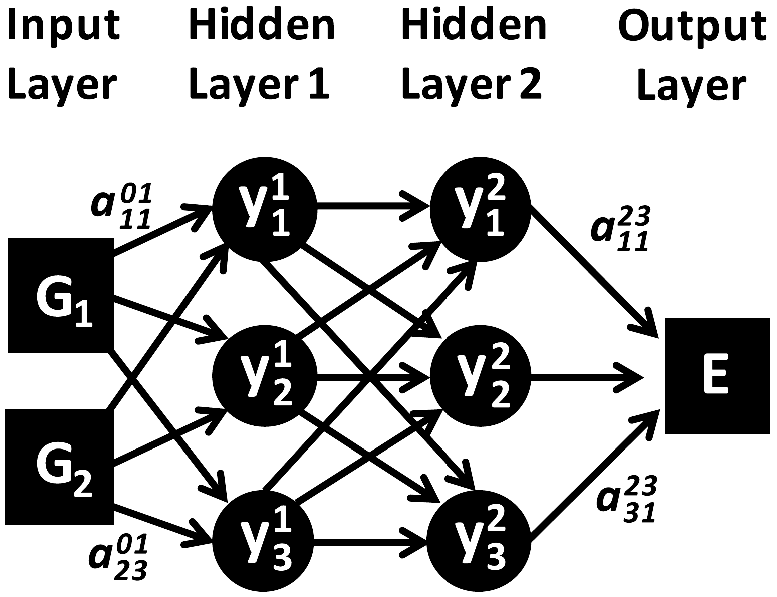
\includegraphics[width=\columnwidth]{MLP-NN.png}

                \tiny{Behler (2016). \textit{The Journal of chemical physics}}
            \end{center}

            \pause
        
            \column{0.7\textwidth}
            \begin{center}
                \tiny{Behler (2017). \textit{Angewandte Chemie International}}

                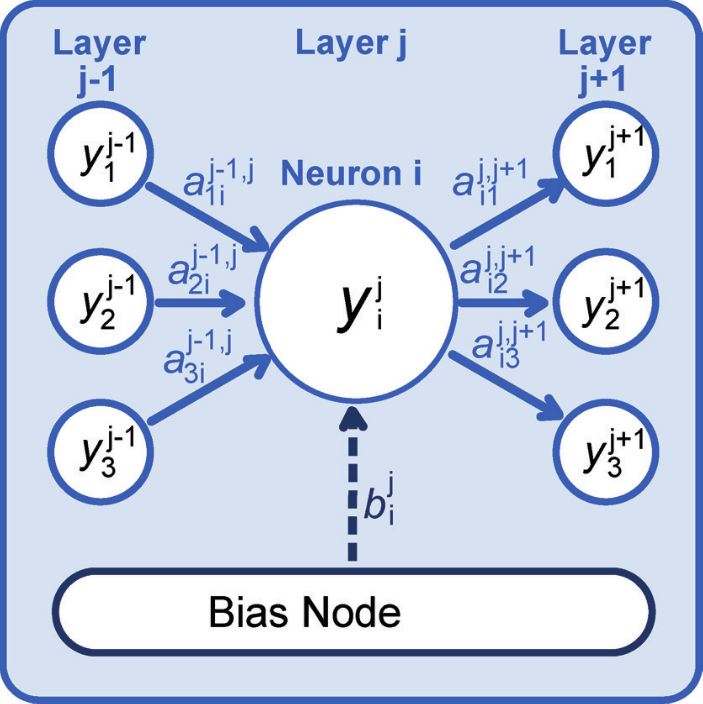
\includegraphics[width=0.4\columnwidth]{MLP-NN-node.png}
            \end{center}
            $$
            E = f\left(
                b_1^3 + \sum_{k=1}^3 a_{k1}^{23} \cdot f\left(
                    b_k^2 + \sum_{j=1}^3 a_{jk}^{12} \cdot f\left(
                        b_j^1 + \sum_{i=1}^2 G_i \cdot a_{ij}^{01}
                    \right)
                \right)
            \right)
            $$

        \end{columns}

    \end{frame}
    
    \begin{frame}
        \frametitle{Potenciales interatómicos de aprendizaje automático}

        \begin{columns}
            \column{0.3\textwidth}
            \textbf{Redes neuronales (NN)}
            \begin{itemize}
                \item Red neuronal feed-forward.
                \item Flexibilidad funcional para representar funciones
                    arbitrarias.
            \end{itemize}

            \begin{center}
                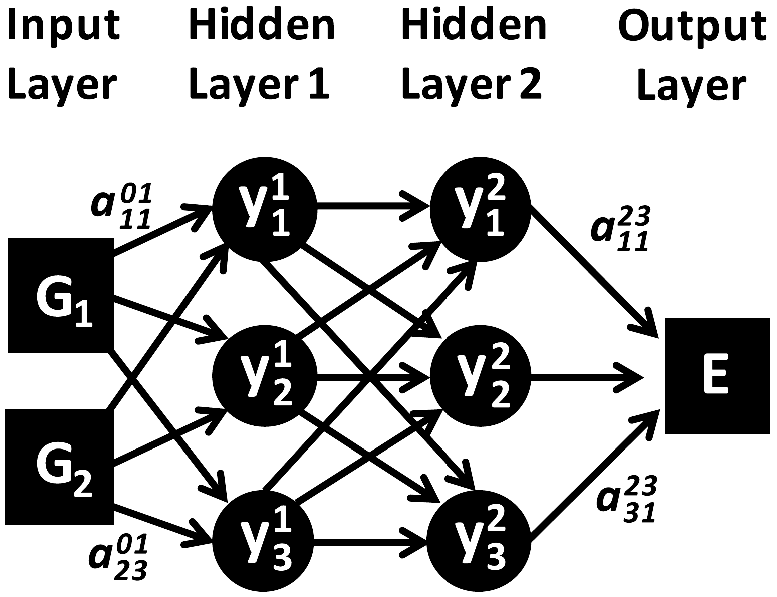
\includegraphics[width=\columnwidth]{MLP-NN.png}

                \tiny{Behler (2016). \textit{The Journal of chemical physics}}
            \end{center}
        
            \column{0.7\textwidth}
            Los parámetros de peso se determinan usando las energías y las fuerzas
            de cálculos previos de la estructura electrónica en un proceso 
            iterativo de optimización por el gradiente.

            \

            Una vez obtenida toda la información de la base de datos la misma es
            evaluada durante la simulación directamente.

        \end{columns}

    \end{frame}
    
    \begin{frame}
        \frametitle{Potenciales interatómicos de aprendizaje automático}
        
        \textbf{Potenciales de aproximación gaussiana (GAP)}: Son obtenidos 
        combinando un descriptor adecuado y un kernel para obtener una conexión 
        entre la estructura y la energía:

        \begin{columns}
            \column{0.5\textwidth}
            $$
            E_i(\mathbf{q}_i) = \sum_{j=1}^{N_{basis}} \alpha_j \chi_j(\mathbf{q}_j).
            $$

            \column{0.5\textwidth}
            $$
            E_i = \sum_{j=1}^{N_{train}} \alpha_j K(\mathbf{q}, \mathbf{q}_j).
            $$
        \end{columns}

        \ \pause

        La energía atómica,
        $$
        E_i  = \sum_{n=1}^{N_{ref}} \alpha_n e^{-\frac{1}{2}\cdot\sum_{l=1}^L [(\mathbf{q}_l - \mathbf{q}_{n,l}) / \theta_l]^2},
        $$

        \ \pause

        es una suma pesada sobre las energías de los entornos atómicos conocidos
        en los datos de referencia, que tienen que estar disponibles a la hora
        de utilizar este potencial.

    \end{frame}

    %%%% APLICACIONES %%%%
    \section{Aplicaciones en baterías de litio}

    \subsection{Li$_3$PO$_4$}
    \begin{frame}
        \begin{center}
            {\huge Li$_3$PO$_4$}
        \end{center}
        \tiny{
            Li, W., Ando, Y., Minamitani, E., \& Watanabe, S. (2017). 
            Study of Li atom diffusion in amorphous Li3PO4 with neural 
            network potential. \textit{The Journal of chemical physics}, 
            147(21), 214106.
        }
    \end{frame}

    \begin{frame}
        \frametitle{Aplicaciones en baterías de litio: Li$_3$PO$_4$}
            
        El \textbf{fosfato de litio} (a-Li$_3$PO$_4$) es un electrolito sólido 
        clásico, que puede ser fabricado en películas delgadas.
            
        \begin{columns}
            \column{0.3\textwidth}
            \begin{center}
                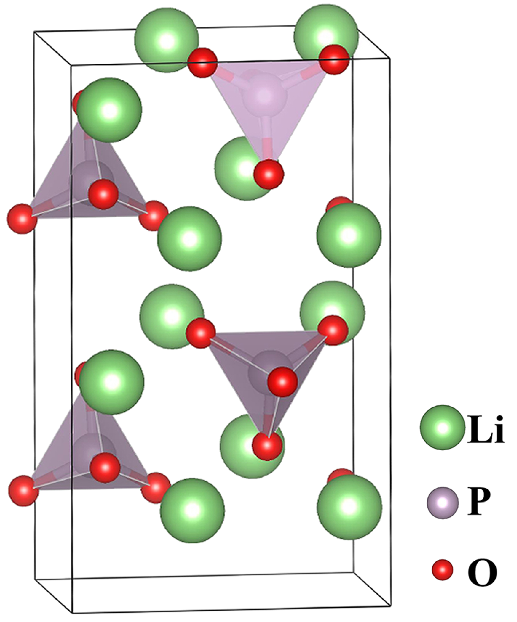
\includegraphics[width=\columnwidth]{Li3PO4-estructura.png}
            \end{center}
        
            \pause 

            \column{0.7\textwidth}
            \textbf{Base de datos}:
            \begin{itemize}
                \item Las energías de referencia fueron calculadas con DFT (VASP).
                \item Celdas de 15-16, 29-32, 61-64 átomos.
                \item Convergencia de la energía en 1 meV/átomo.

                \pause

                \item Se utilizaron distintas estructuras (38592) además de las 
                    cristalinas:
                    \begin{enumerate}
                        \item \textit{frames} de trayectorias de MD entre 300 K
                            y 4000 K,
                        \item Estructuras con defectos, extrayendo átomos de Li o
                            una unidad Li$_2$O de manera aleatoria, de los 
                            \textit{frames} anteriores.
                        \item Imágenes intermedias de NEB.
                    \end{enumerate}
                \item De las 38592 estructuras, se utilizaron 30874 
                    ($\approx$80\%) en el entrenamiento y 7718 ($\approx$20\%) 
                    para testear.
            \end{itemize}
        \end{columns}

    \end{frame}
    
    \begin{frame}
        \frametitle{Aplicaciones en baterías de litio: Li$_3$PO$_4$}
            
        \textbf{Preparación de los datos y entrenamiento}:
        \begin{itemize}
            \item Se usaron los dos tipos de descriptores ASCF, radial y angular, 
                con un radio de corte de 7\AA.
            \item Redes neuronales para cada especie de átomo con 2 capas ocultas
                y 15 nodos en cada una de ellas. Tangente hiperbólica como función
                de activación. Función de activación lineal en el nodo de salida.
        \end{itemize}

        \pause

        \begin{columns}
            \column{0.2\textwidth}
            \begin{center}
                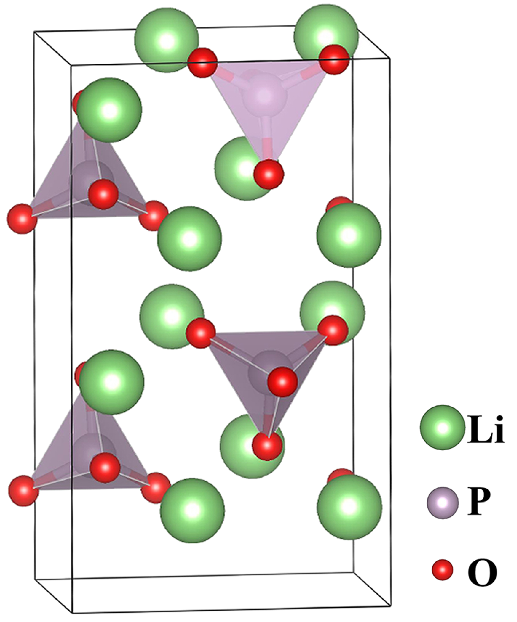
\includegraphics[width=\columnwidth]{Li3PO4-estructura.png}
            \end{center}

            \column{0.8\textwidth}
            \begin{center}
                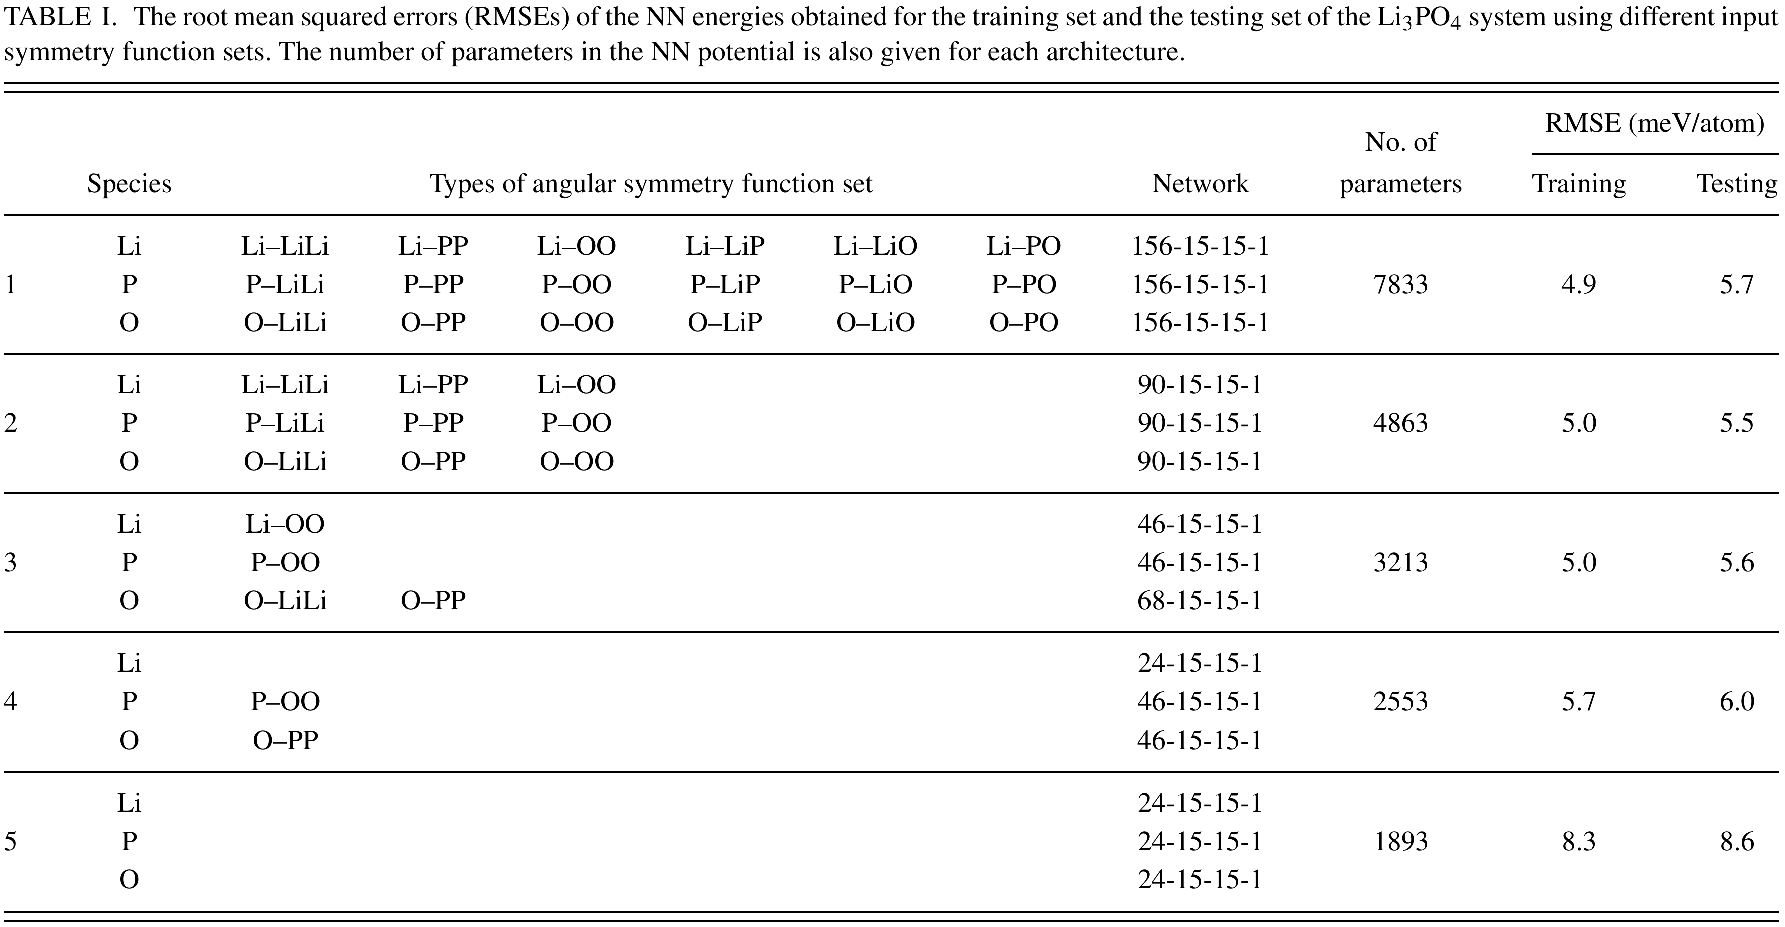
\includegraphics[width=0.7\columnwidth]{Li3PO4-rmse.png}
            \end{center}
        \end{columns}

    \end{frame}
    
    \begin{frame}
        \frametitle{Aplicaciones en baterías de litio: Li$_3$PO$_4$}

        \begin{center}
            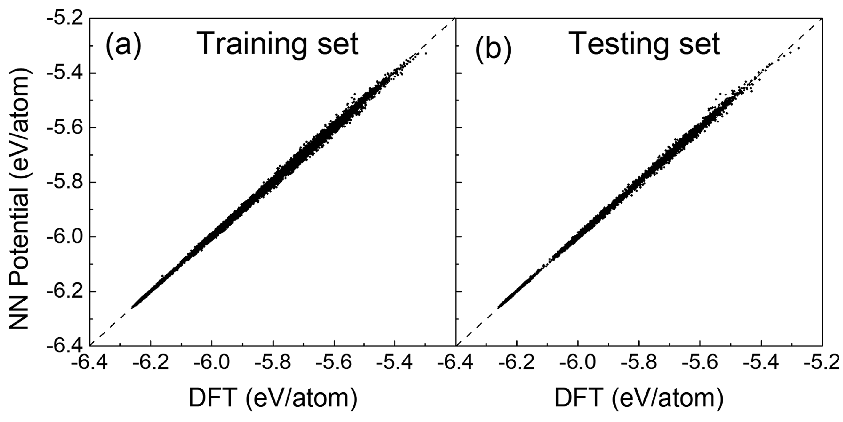
\includegraphics[width=0.6\textwidth]{Li3PO4-training_testing.png}

            {\tiny Li \textit{et al.} (2017). \textit{The Journal of chemical
            physics}}
        \end{center}

        RMSE de 5.0 meV/átomo y 5.6 meV/átomo para los conjuntos de entrenamiento
        y testeo, respectivamente.

    \end{frame}

    \begin{frame}
        \frametitle{Aplicaciones en baterías de litio: Li$_3$PO$_4$}
         
        \textbf{Uso en simulaciones}

        Templado simulado para obtener a-Li$_3$PO$_4$:
        \begin{enumerate}
            \item \textit{melting} a 6000 K por 15 ps de $\gamma$-Li$_3$PO$_4$, 
            \item \textit{quenching} de 6000 K a 300 K a una tasa de 1 K/fs.
        \end{enumerate}

        \pause

        \begin{columns}
            \column{0.5\textwidth}
            Energía de formación de vacancias
            $$
            E_f = E[V_{Li}] - E[bulk] + \mu_{Li}
            $$

            \pause 

            \column{0.5\textwidth}
            \begin{center}
                \tiny{Li \textit{et al.} (2017). \textit{The Journal of chemical
                physics}}

                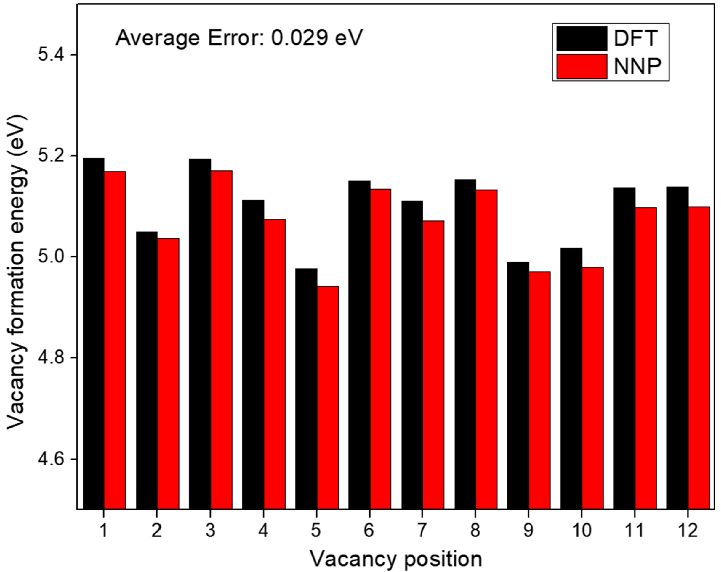
\includegraphics[width=0.8\columnwidth]{Li3PO4-vacancias.png}
            \end{center}
        \end{columns}

    \end{frame}
    
    \begin{frame}
        \frametitle{Aplicaciones en baterías de litio: Li$_3$PO$_4$}
            
        \textbf{Uso en simulaciones}

        Difusión de Li en la estructura con una vacancia.
        
        \begin{columns}
            \column{0.3\textwidth}
            \begin{center}
                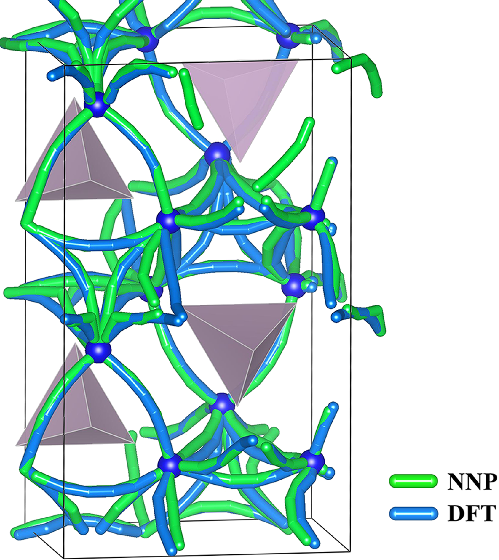
\includegraphics[width=\columnwidth]{Li3PO4-neb.png}
            \end{center}
            \tiny{Li \textit{et al.} (2017). \textit{The Journal of chemical
            physics}}

            \column{0.7\textwidth}
            Se obtuvieron 46 caminos de migración para los átomos de Li mediante
            la técnica de NEB.

            \ \pause

            La barrera de energía promedio con DFT es de 0.58 eV y con NN es 
            0.57 eV.
        \end{columns}

    \end{frame}
    
    \begin{frame}
        \frametitle{Aplicaciones en baterías de litio: Li$_3$PO$_4$}
            
        \textbf{Uso en simulaciones}

        Difusión de Li en la estructura con una vacancia.
        
        \begin{columns}
            \column{0.6\textwidth}
            Usando los NEBs obtenidos, se realizan simulaciones de kMC
            $$
            p = k \exp \left( - \frac{\Delta E_{ij}}{k_B T} \right),
            $$
            $k = 10^{13} s^{-1}$

            $100 \times 10^6$ MC eventos realizados a distintas temperaturas.

            \pause

            $$
            D = \frac{1}{6} \lim_{\Delta t \rightarrow \infty} \langle MSD \rangle
            = \frac{1}{6} \lim_{\Delta t \rightarrow \infty} \frac{\langle (r_i(t_0 + \Delta t) - r_i(t_0))^2 \rangle}{\Delta t}
            $$

            \pause 

            \column{0.4\textwidth}
            Energías de activación: 0.602 eV y 0.561 eV, para los NEBs resultantes 
            de NN y DFT.
            \begin{center}
                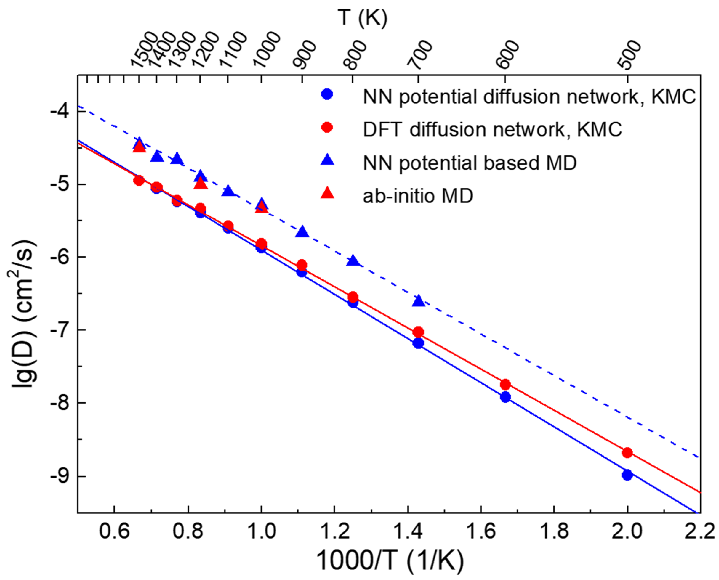
\includegraphics[width=0.9\columnwidth]{Li3PO4-kMC-arrhenius.png}
            \end{center}
            \tiny{Li \textit{et al.} (2017). \textit{The Journal of chemical
            physics}}
        \end{columns}

    \end{frame}
    
    \begin{frame}
        \frametitle{Aplicaciones en baterías de litio: Li$_3$PO$_4$}
            
        \textbf{Uso en simulaciones}

        Difusión de Li en la estructura con una vacancia.
        
        \begin{columns}
            \column{0.6\textwidth}
            Simulaciones de dinámica molecular (\textit{ab-initio} y NN):
            \begin{itemize}
                \item ensamble NVT,
                \item paso temporal de 2 fs,
                \item equilibración de 10 ps,
                \item 50 ps para los cálculos (1 ns para NN).
            \end{itemize}

            \column{0.4\textwidth}
            Energías de activación: 0.59 eV para MD NN (0.602 eV y 0.561 eV en 
            kMC). 
            \begin{center}
                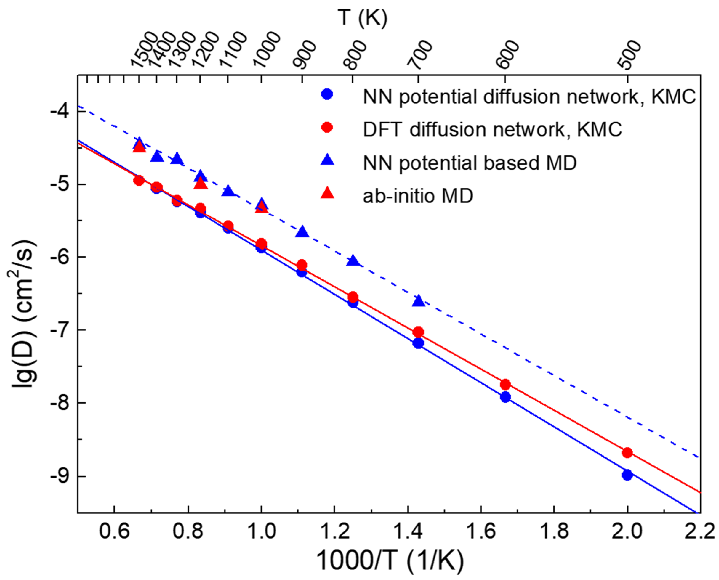
\includegraphics[width=0.9\columnwidth]{Li3PO4-kMC-arrhenius.png}
            \end{center}
            \tiny{Li \textit{et al.} (2017). \textit{The Journal of chemical
            physics}}
        \end{columns}

    \end{frame}
    
    \begin{frame}
        \frametitle{Aplicaciones en baterías de litio: Li$_3$PO$_4$}
            
        \textbf{Uso en simulaciones}

        Difusión de Li en la estructura con una vacancia.
        
        \begin{columns}
            \column{0.6\textwidth}
            Simulación de dinámica molecular con el potencial NN:
            \begin{itemize}
                \item a-Li$_{2.906}$PO$_4$,
                \item 1006 átomos,
                \item 100 ps,
                \item 600 K, 700 K, 800 K, 1000 K, 1200 K.
            \end{itemize}

            Energía de activación obtenida: 0.55 eV

            \column{0.4\textwidth}
            Energías de activación: 0.58 eV (ion-exchange), 0.57 eV (mask) y
            0.55 eV (impedance spectroscopy).
            \begin{center}
                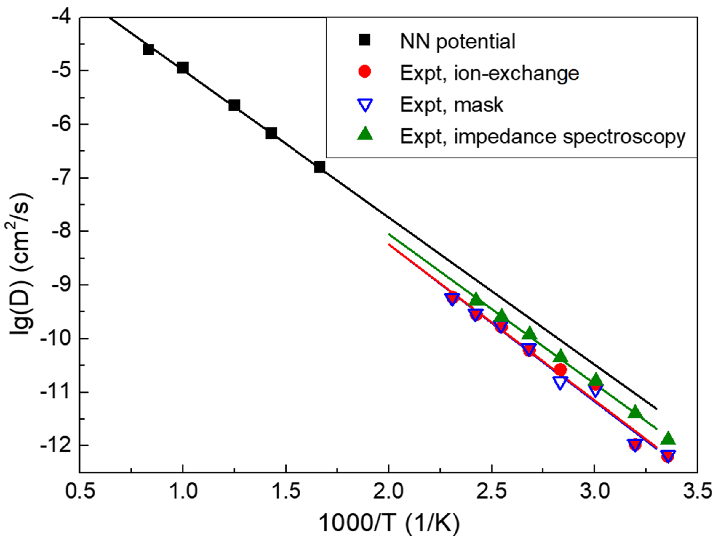
\includegraphics[width=0.9\columnwidth]{Li3PO4-MD-arrhenius.png}
            \end{center}
            \tiny{Li \textit{et al.} (2017). \textit{The Journal of chemical
            physics}}
        \end{columns}

    \end{frame}

    \subsection{Li$_x$C}
    \begin{frame}
        \begin{center}
            {\huge Li$_x$C}
        \end{center}
        \tiny{
            Fujikake, S., Deringer, V. L., Lee, T. H., Krynski, M., 
            Elliott, S. R., \& Csányi, G. (2018). Gaussian approximation 
            potential modeling of lithium intercalation in carbon 
            nanostructures. \textit{The Journal of chemical physics}, 148(24), 241714.
        }
    \end{frame}
    
    \begin{frame}
        \frametitle{Aplicaciones en baterías de litio: Li$_x$C}
            
        Los ánodos de las baterías de litio suelen ser de \textbf{grafito} u otras
        nanoestructuras de carbono.
        
        \begin{columns}
            \column{0.4\textwidth}
            \begin{center}
                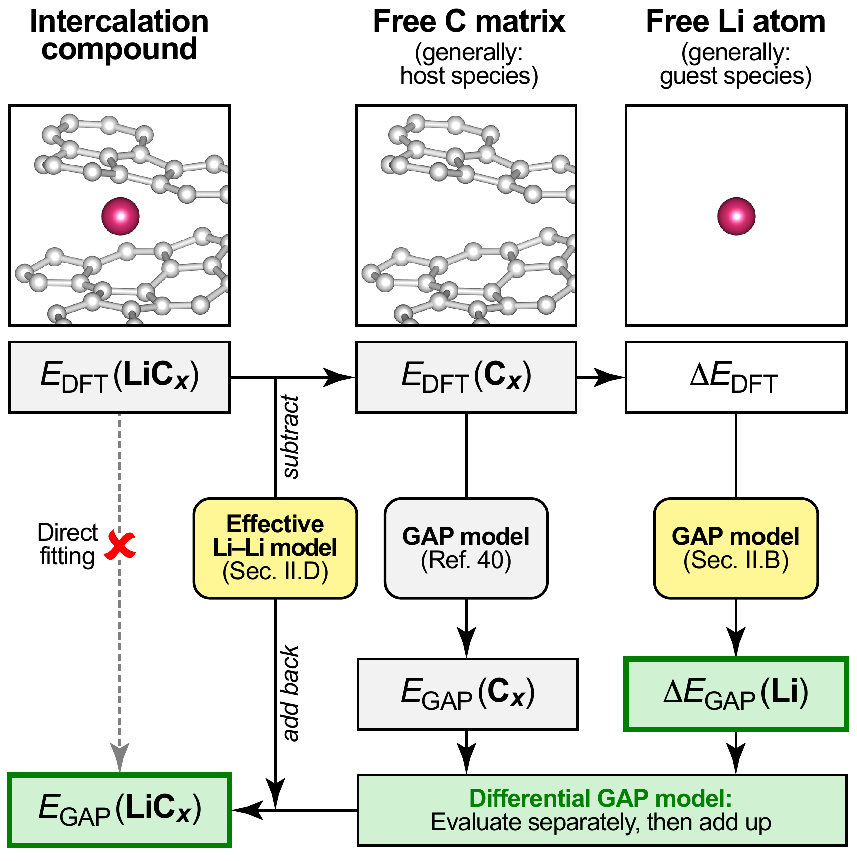
\includegraphics[width=0.9\columnwidth]{LiC-metodo.png}
            \end{center}
            \tiny{Fujikake \textit{et al.} (2018). \textit{The Journal of chemical
            physics}}

            \pause

            \column{0.6\textwidth}
            Ya está desarrollado un potencial GAP para estructuras de carbono, 
            el objetivo de este trabajo es agregar la interacción de los átomos
            de Li como una extensión.
            
            \ \pause

            Fitean las diferencias en energía que se dan al insertar Li,
            $$
            \Delta E_{DFT} = E_{DFT}(Li_xC) - E_{DFT}(C_x) - E_{DFT}(Li),
            $$
            con un potencial GAP.

        \end{columns}

    \end{frame}
    
    \begin{frame}
        \frametitle{Aplicaciones en baterías de litio: Li$_x$C}
            
        Los ánodos de las baterías de litio suelen ser de \textbf{grafito} u otras
        nanoestructuras de carbono.
        
        \begin{columns}
            \column{0.4\textwidth}
            \begin{center}
                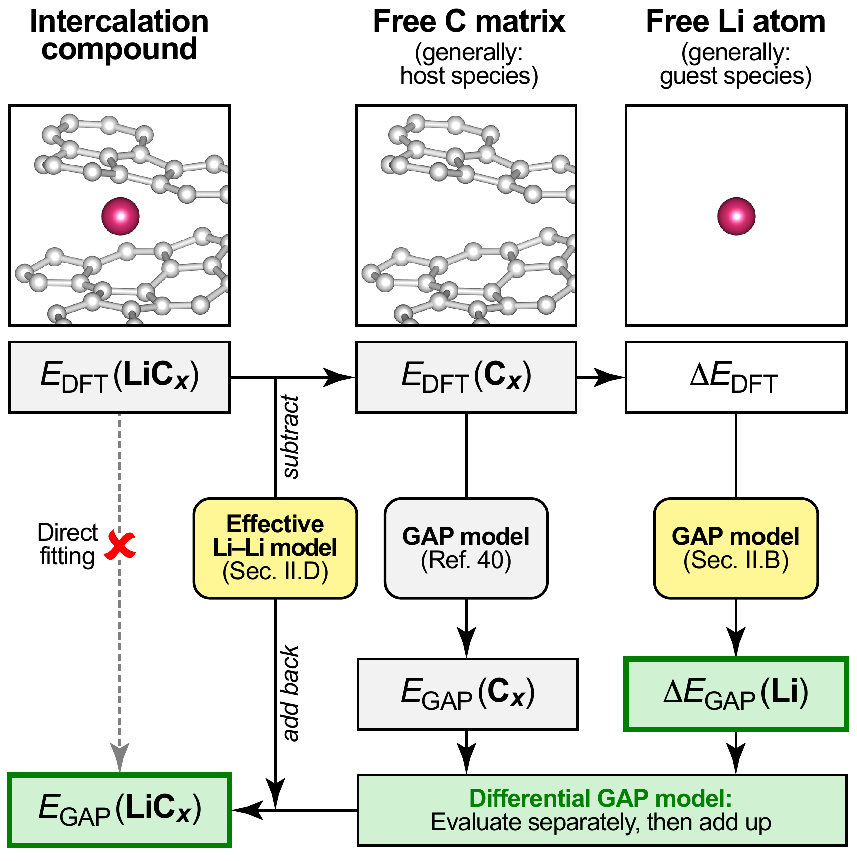
\includegraphics[width=0.9\columnwidth]{LiC-metodo.png}
            \end{center}
            \tiny{Fujikake \textit{et al.} (2018). \textit{The Journal of chemical
            physics}}

            \column{0.6\textwidth}
            Cuatro descriptores:
            \begin{enumerate}
                \item Un término de dos cuerpos para la interacción Li-C, 
                \item otro para las interacciones Li-Li,
                \item un término de tres cuerpos para los ángulos de un átomo 
                    central de Li y dos vecinos de C (hasta acá kernel gaussiano),
                \item un término de muchos cuerpos para todos los vecinos de C
                    de un átomo de Li hasta un radio de corte (SOAP).
            \end{enumerate}
        \end{columns}

    \end{frame}
    
    \begin{frame}
        \frametitle{Aplicaciones en baterías de litio: Li$_x$C}
        
        \begin{columns}
            \column{0.6\textwidth}
            El método directo no da buenos resultados para la interacción Li-Li.

            % Esto se debe a que el cambio de energía al insertar un átomo de Li
            % es $\approx$1 eV, mientras que la interacción Li-Li es $\approx$0.1 eV.

            \ \pause 

            Se introduce un potencial efectivo para la interacción Li-Li (GAP de 
            2 cuerpos).

            \column{0.4\textwidth}
            \begin{center}
                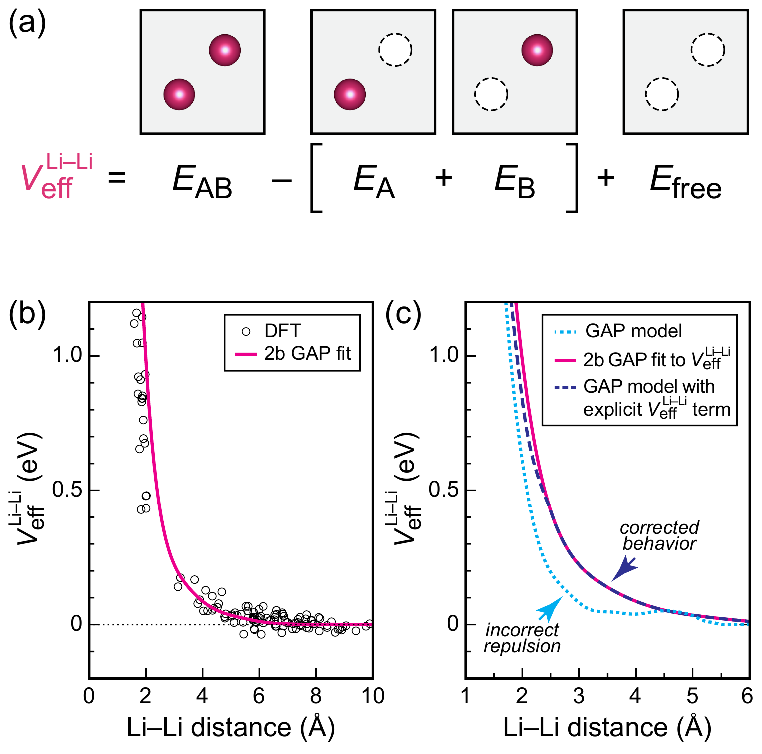
\includegraphics[width=\columnwidth]{LiC-LiLi_efectivo.png}
            \end{center}
            \tiny{Fujikake \textit{et al.} (2018). \textit{The Journal of chemical
            physics}}
        \end{columns}

    \end{frame}

    \begin{frame}
        \frametitle{Aplicaciones en baterías de litio: Li$_x$C}
        
        \begin{columns}
            \column{0.4\textwidth}
            \begin{center}
                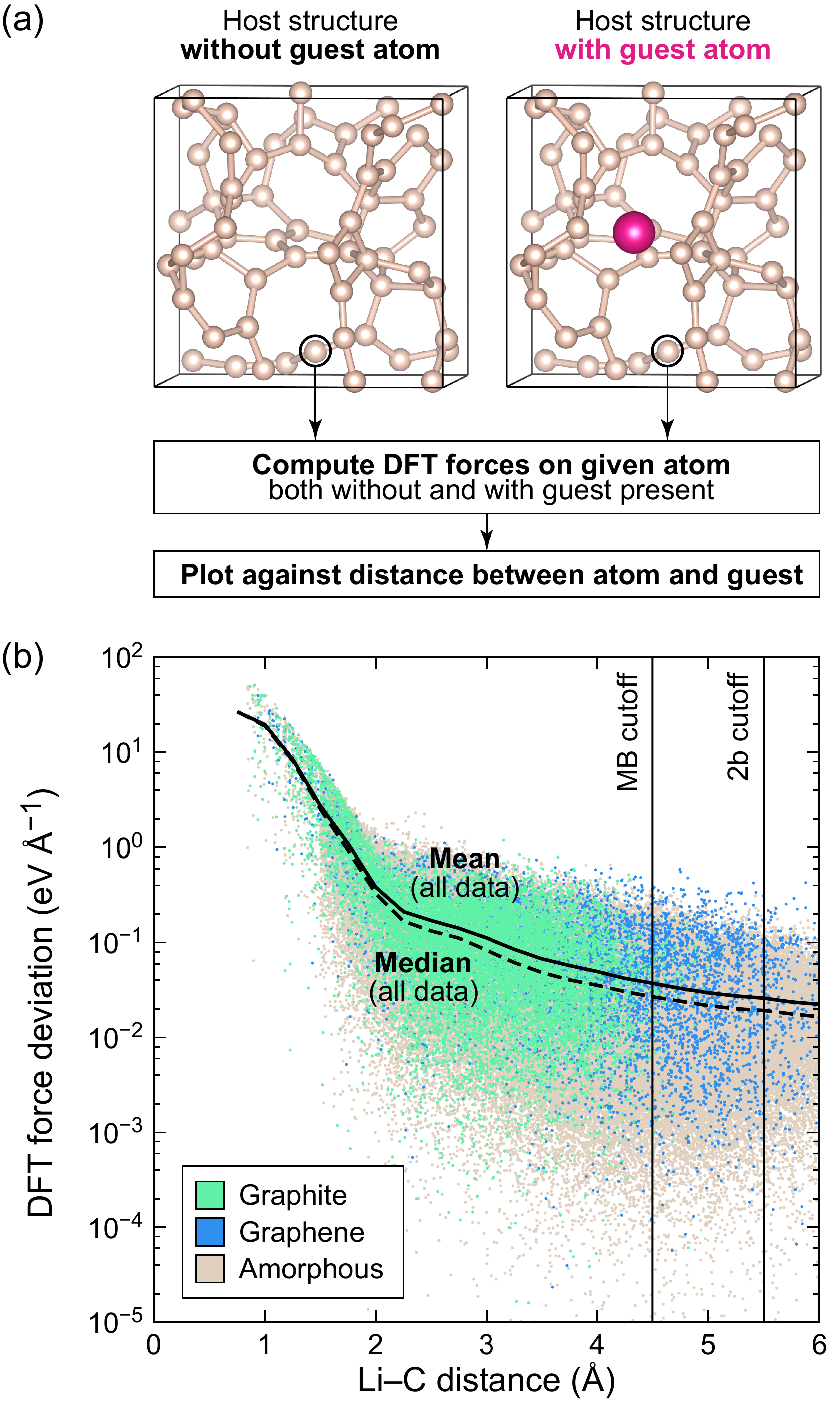
\includegraphics[width=0.7\columnwidth]{LiC-fuerza_1_atomo_de_Li.png}
            \end{center}

            \column{0.6\textwidth}
            {\tiny Fujikake \textit{et al.} (2018). \textit{The Journal of chemical
            physics}}

            \

            \

            \textbf{Base de datos}:
            \begin{itemize}
                \item Átomos de Li en posiciones aleatorias de estructuras de:
                    \begin{enumerate}
                        \item grafito desordenado (24 átomos y 561 estructuras), 
                        \item grafeno (24 átomos y 192 estructuras), y
                        \item carbono amorfo (64 átomos y 1664 estructuras)
                    \end{enumerate}
                    hasta un 10\% de concentración.
            \end{itemize}
        \end{columns}

    \end{frame}
    
    \begin{frame}
        \frametitle{Aplicaciones en baterías de litio: Li$_x$C}
        
        \begin{columns}
            \column{0.5\textwidth}
            \begin{center}
                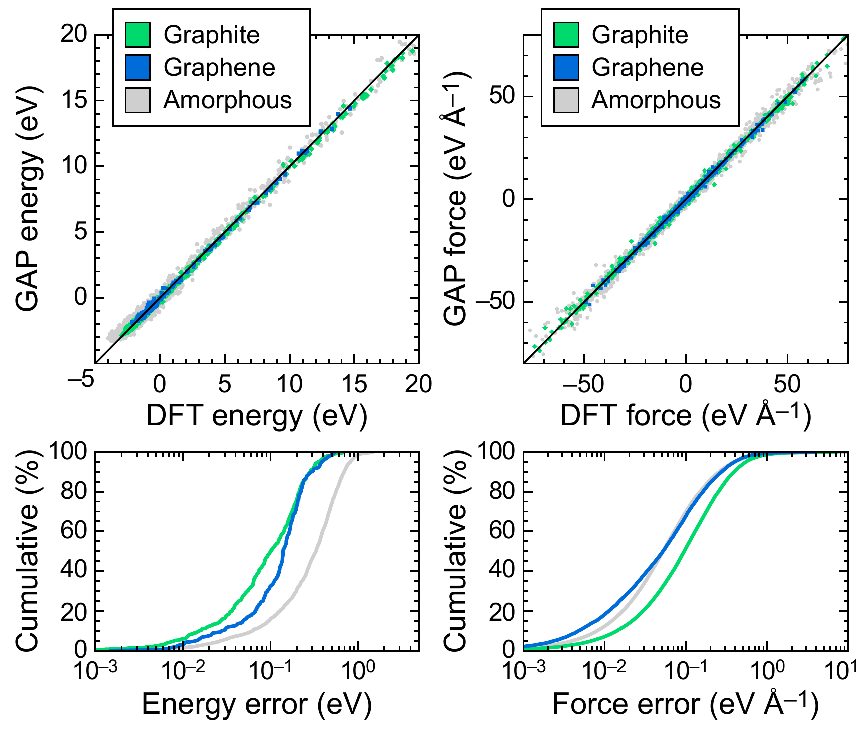
\includegraphics[width=\columnwidth]{LiC-training_testing.png}
            \end{center}
            \tiny{Fujikake \textit{et al.} (2018). \textit{The Journal of chemical
            physics}}

            \column{0.5\textwidth}
            RMSE (MAE) de la energía de intercalación de Li: 0.37 (0.29) eV/átomo

            \ \pause

            Dividido por grupos (RMSE):
            \begin{itemize}
                \item a-C: 0.43 eV/átomo,
                \item grafito: 0.17 eV/átomo.
                \item grafeno: 0.19 eV/átomo.
            \end{itemize}
        \end{columns}
    \end{frame}
    
    %\begin{frame}
    %    \frametitle{Aplicaciones en baterías de litio: Li$_x$C}
    %
    %    \textbf{Absorsión de un átomo de Li y difusión entre dos mínimos de 
    %    potencial}
    %    
    %    \begin{center}
    %        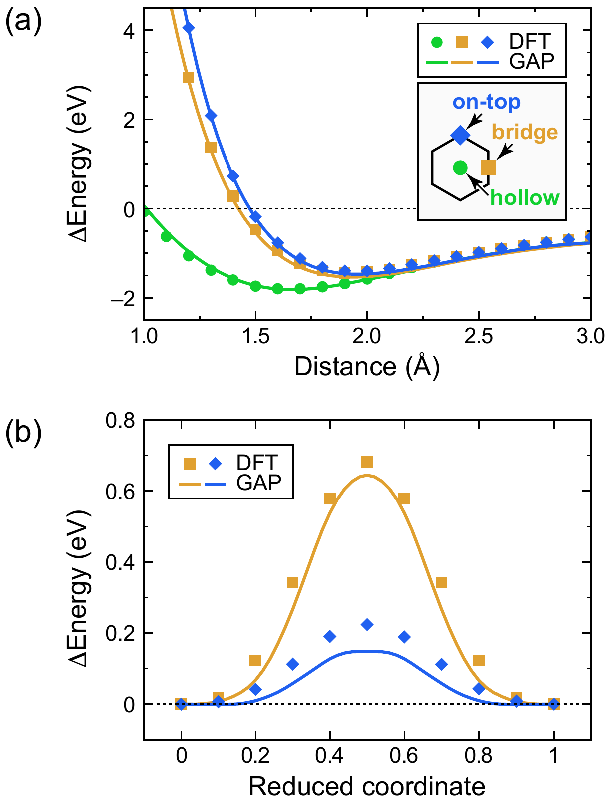
\includegraphics[width=0.3\textwidth]{LiC-sites.png}
    %    \end{center}
    %    \tiny{Fujikake \textit{et al.} (2018). \textit{The Journal of chemical
    %    physics}}
    %\end{frame}
    
    \begin{frame}
        \frametitle{Aplicaciones en baterías de litio: Li$_x$C}

        \textbf{Simulaciones de dinámica molecular}

        4 átomos de Li en una estructura de grafito desordenada.
        
        \begin{columns}
            \column{0.5\textwidth}
            \begin{itemize}
                \item Temperatura: 1000 K
                \item Paso temporal: 1 fs
                \item Tiempo de equilibración: 25 ps 
                \item Tiempo de muestreo: 50 ps
            \end{itemize}

            \ \pause

            Número de coordinación Li-C: 7.3 (DFT), 6.9 (GAP).

            \column{0.5\textwidth}
            \begin{center}
                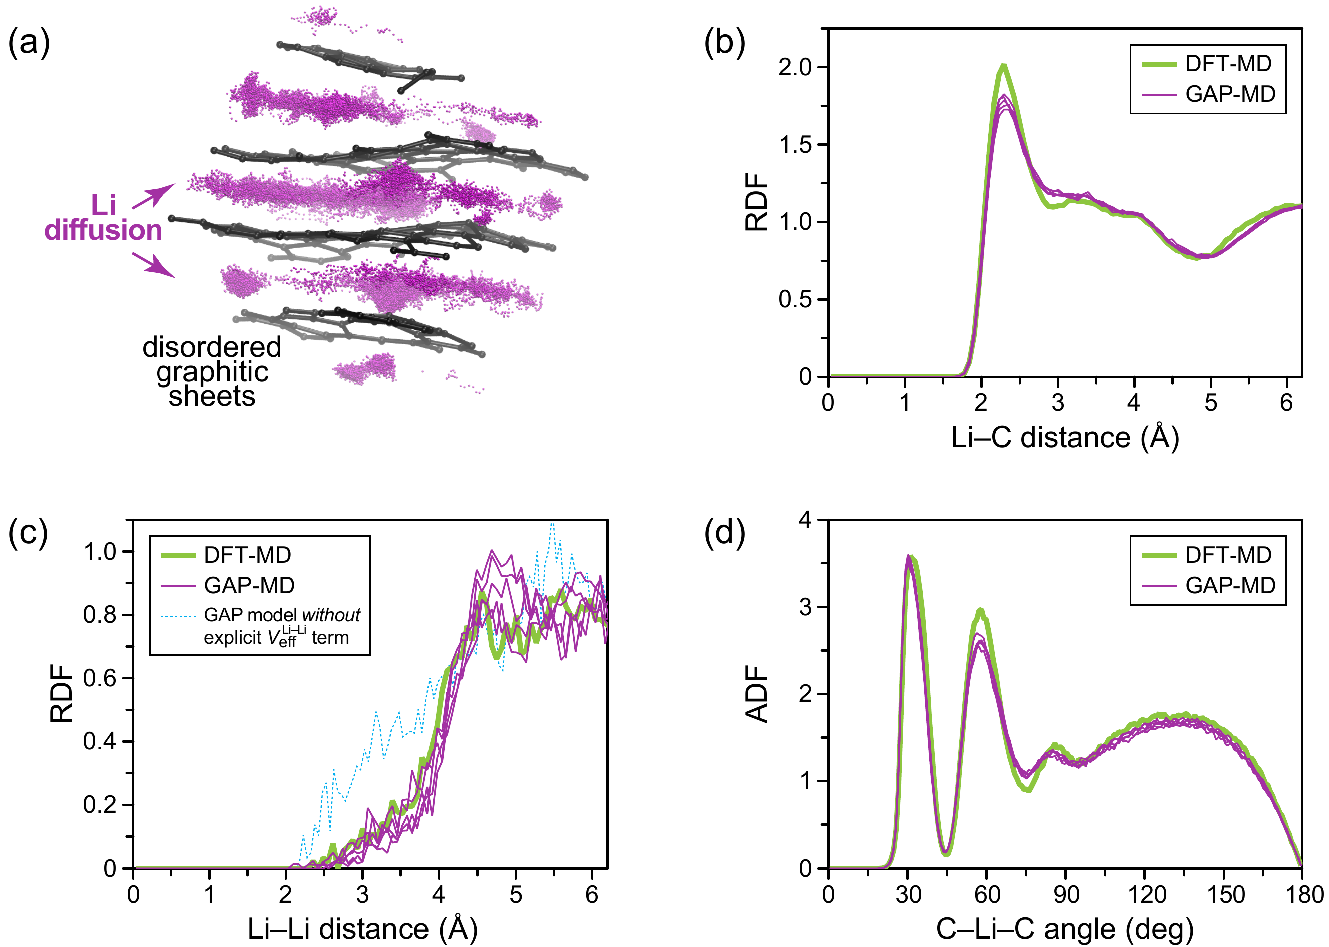
\includegraphics[width=\columnwidth]{LiC-MD-results.png}
            \end{center}
            \tiny{Fujikake \textit{et al.} (2018). \textit{The Journal of chemical
            physics}}
        \end{columns}
    \end{frame}
    
    \begin{frame}
        \frametitle{Aplicaciones en baterías de litio: Li$_x$C}

        \textbf{Simulaciones de dinámica molecular}

        4 átomos de Li en una estructura de grafito desordenada.
        
        \begin{columns}
            \column{0.35\textwidth}
            \begin{center}
                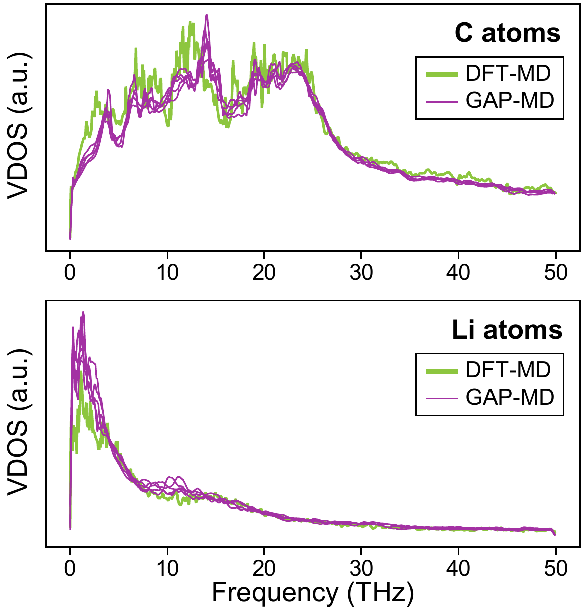
\includegraphics[width=\columnwidth]{LiC-VDOS.png}
            \end{center}
            \tiny{Fujikake \textit{et al.} (2018). \textit{The Journal of chemical
            physics}}
            
            \column{0.65\textwidth}
            \textit{Vibrational density of states} usando la función de 
            autocorrelación de las velocidades.
        \end{columns}
    \end{frame}

    \subsection{Li$_x$Si}

    \begin{frame}
        \begin{center}
            {\huge Li$_x$Si}
        \end{center}
        \tiny{
            Artrith, N., Urban, A., \& Ceder, G. (2018). Constructing 
            first-principles phase diagrams of amorphous Li x Si using 
            machine-learning-assisted sampling with an evolutionary algorithm. 
            \textit{The Journal of chemical physics}, 148(24), 241711.
        }
    \end{frame}
    
    \begin{frame}
        \frametitle{Aplicaciones en baterías de litio: Li$_x$Si}
        
        El \textbf{silicio} amorfo es un potencial material de ánodo de alta
        capacidad para las baterías de litio.
        
        \begin{columns}
            \column{0.65\textwidth}
            \begin{center}
                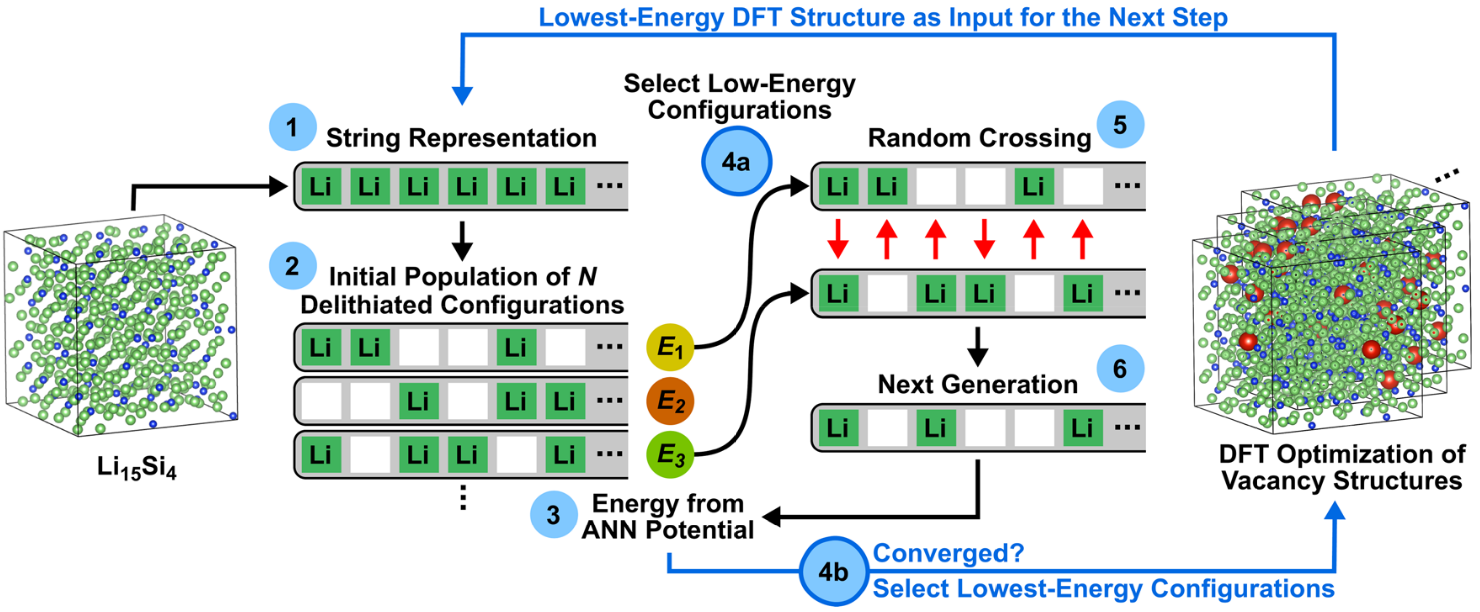
\includegraphics[width=\columnwidth]{LiSi-metodo.png}
            \end{center}
            \tiny{Artrith \textit{et al.} (2018). \textit{The Journal of chemical
            physics}}

            \pause
            
            \column{0.35\textwidth}
            \begin{itemize}
                \item Potencial NN de 2 capas ocultas con 15 nodos cada una.
                \item 90\% / 10\% de datos de referencia DFT para entrenamiento / 
                    testing.
                \item Descriptores: RDF y ADF con $\omega_{Li} = -1$, 
                    $\omega_{Si} = 1$ y $N = 11$ (polinomios de Chebyshev).
            \end{itemize}
        \end{columns}
            
    \end{frame}
    
    \begin{frame}
        \frametitle{Aplicaciones en baterías de litio: Li$_x$Si}
        
        El \textbf{silicio} amorfo es un potencial material de ánodo de alta
        capacidad para las baterías de litio.
        
        \begin{columns}
            \column{0.65\textwidth}
            \begin{center}
                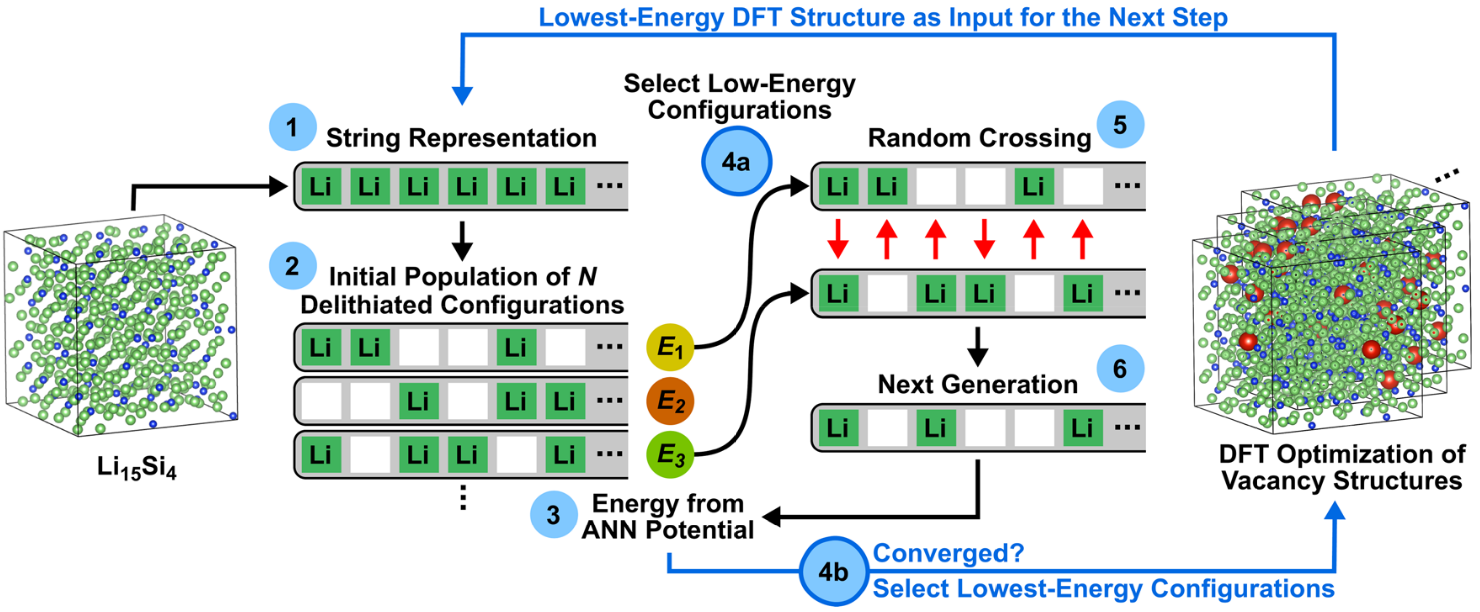
\includegraphics[width=\columnwidth]{LiSi-metodo.png}
            \end{center}
            \tiny{Artrith \textit{et al.} (2018). \textit{The Journal of chemical
            physics}}

            \column{0.35\textwidth}
            \begin{itemize}
                \item Generación de estructuras amorfas:
                    \begin{enumerate}
                        \item Potencial NN con 725 estructuras de DFT (estructuras
                            cristalinas, escaleo isotrópico, vacancias).
                        \item Mediante algoritmos genéticos se busca que átomo 
                            de Li extraer en un proceso de delitiación.
                    \end{enumerate}
            \end{itemize}
        \end{columns}
            
    \end{frame}
    
    \begin{frame}
        \frametitle{Aplicaciones en baterías de litio: Li$_x$Si}
        
        El \textbf{silicio} amorfo es un potencial material de ánodo de alta
        capacidad para las baterías de litio.
        
        \begin{columns}
            \column{0.65\textwidth}
            \begin{center}
                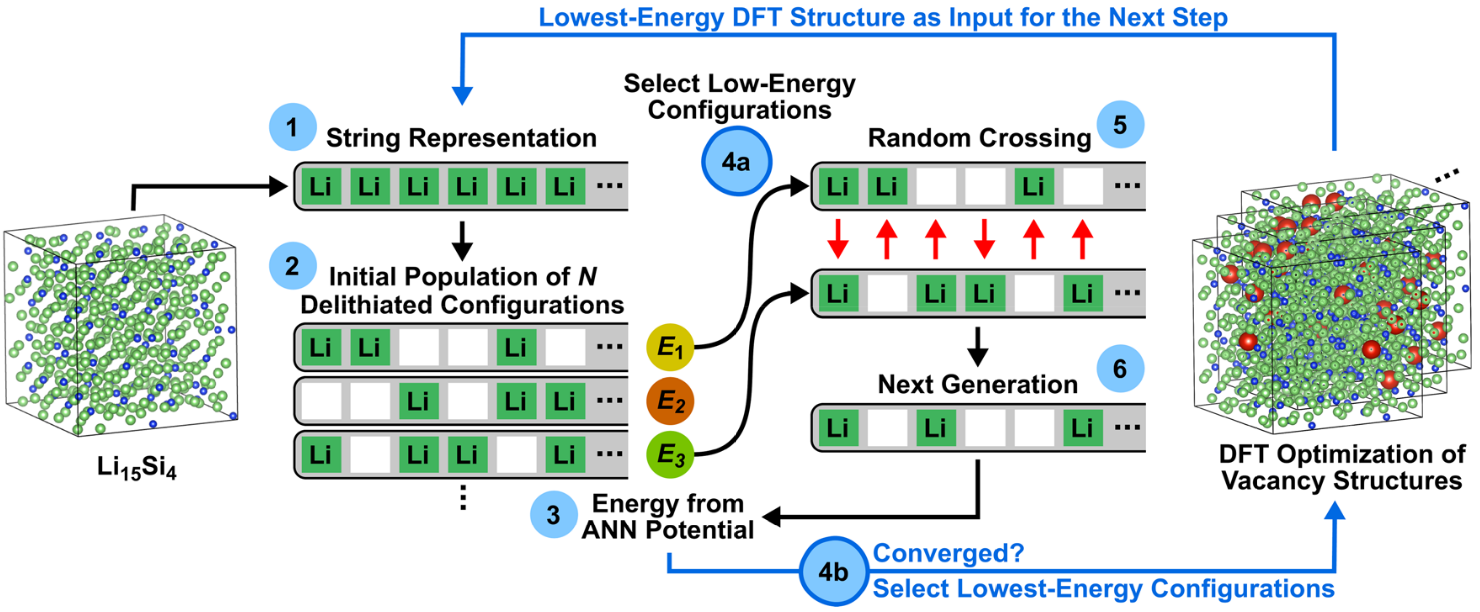
\includegraphics[width=\columnwidth]{LiSi-metodo.png}
            \end{center}
            \tiny{Artrith \textit{et al.} (2018). \textit{The Journal of chemical
            physics}}

            \column{0.35\textwidth}
            Al menos 30 estructuras son optimizadas por DFT para obtener la 
            estructura inicial del siguiente paso.
        \end{columns}
            
    \end{frame}
    
    \begin{frame}
        \frametitle{Aplicaciones en baterías de litio: Li$_x$Si}
        
        El \textbf{silicio} amorfo es un potencial material de ánodo de alta
        capacidad para las baterías de litio.
        
        \begin{columns}
            \column{0.65\textwidth}
            \begin{center}
                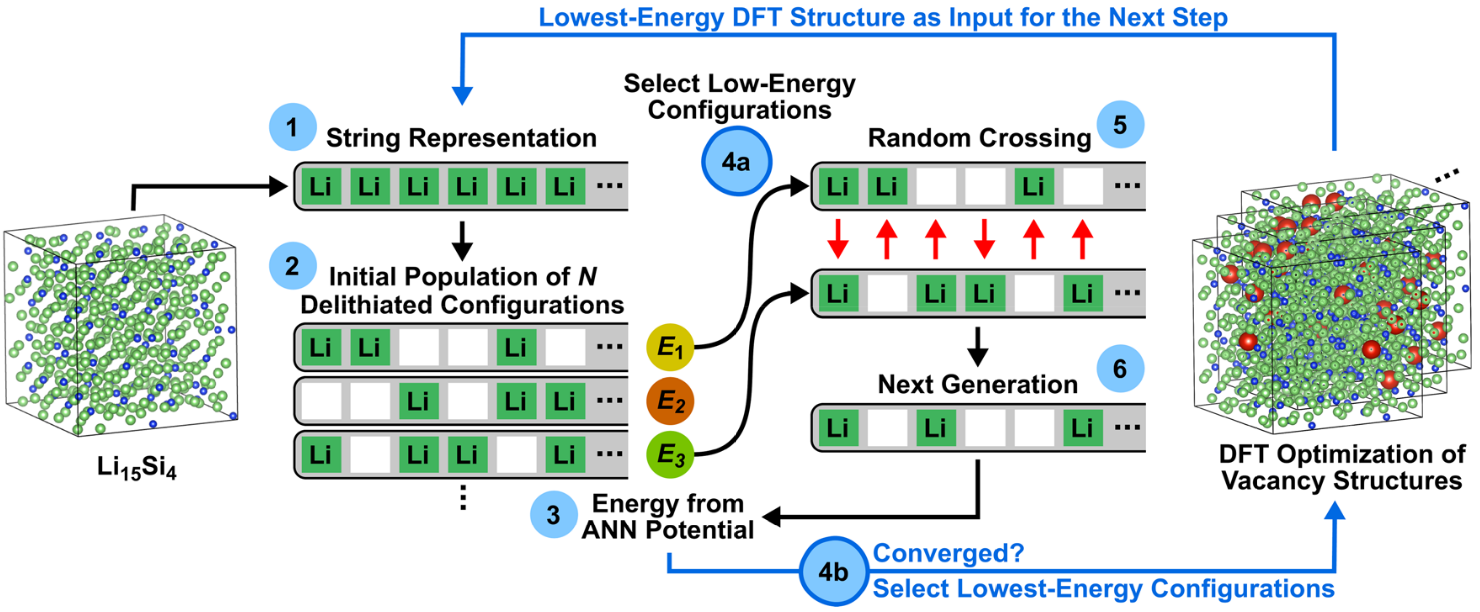
\includegraphics[width=\columnwidth]{LiSi-metodo.png}
            \end{center}
            \tiny{Artrith \textit{et al.} (2018). \textit{The Journal of chemical
            physics}}

            \column{0.35\textwidth}
            \begin{center}
                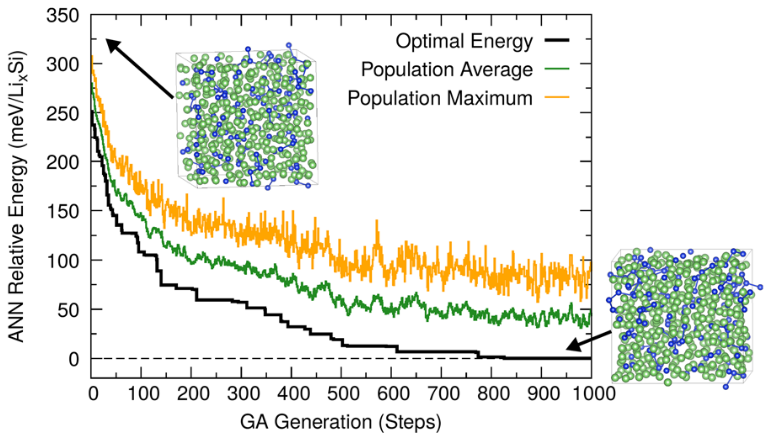
\includegraphics[width=\columnwidth]{LiSi-optimizacion_de_la_energia.png}
            \end{center}
        \end{columns}
            
    \end{frame}
    
    \begin{frame}
        \frametitle{Aplicaciones en baterías de litio: Li$_x$Si}
        
        \textbf{Simulaciones de dinámica molecular}
        
        \begin{columns}
            \column{0.5\textwidth}
            \begin{itemize}
                \item Ensamble NVT, paso temporal de 2 fs y algoritmo de Verlet.
                \item Se reentrenó el potencial con 45000 estructuras de clusters, 
                    bordes y con distintos frames de dinámicas a altas
                    temperaturas.
                \item RMSE: 6.3 (7.7) meV/atom, entrenamiento (testing).
            \end{itemize}

            \pause

            \column{0.5\textwidth}
            \begin{center}
                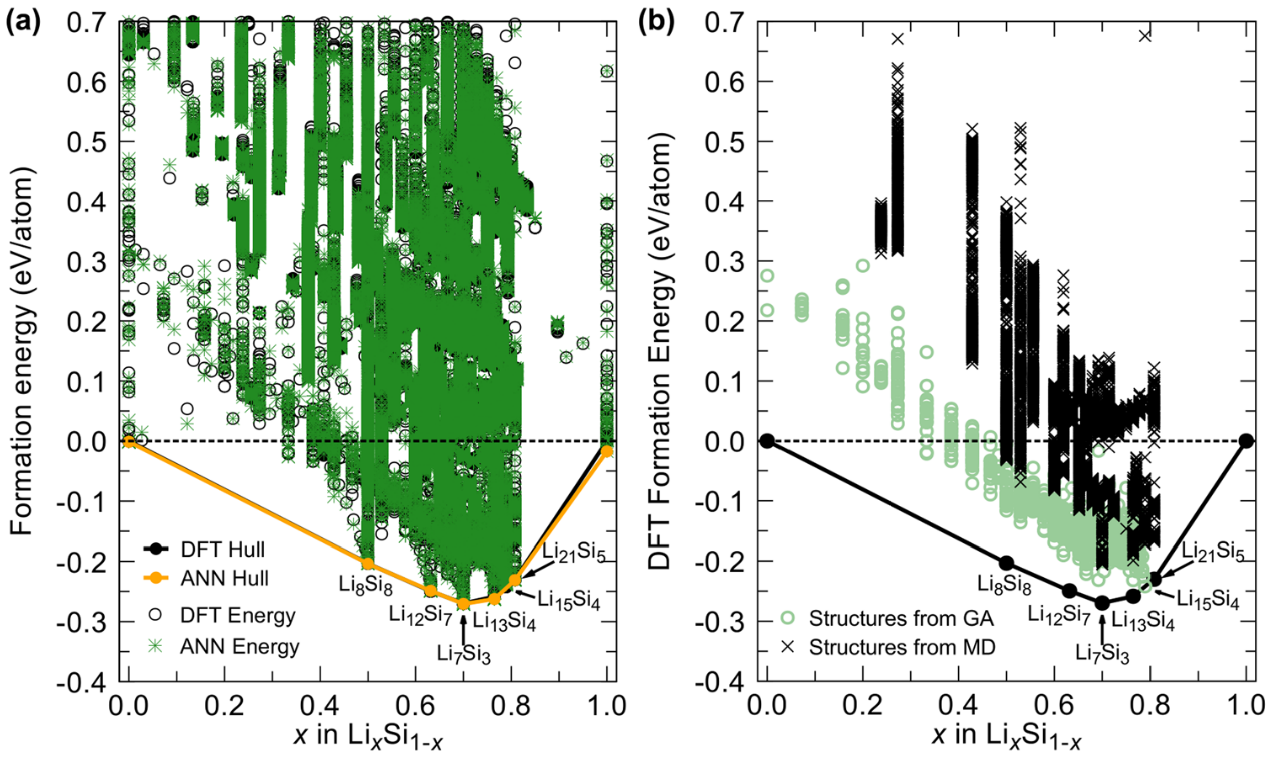
\includegraphics[width=\columnwidth]{LiSi-energias_de_formacion.png}
            \end{center}
            \tiny{Artrith \textit{et al.} (2018). \textit{The Journal of chemical
            physics}}
        \end{columns}
            
    \end{frame}
    
    \begin{frame}
        \frametitle{Aplicaciones en baterías de litio: Li$_x$Si}
        
        \textbf{Simulaciones de dinámica molecular}
        
        \begin{columns}
            \column{0.7\textwidth}
            \begin{center}
                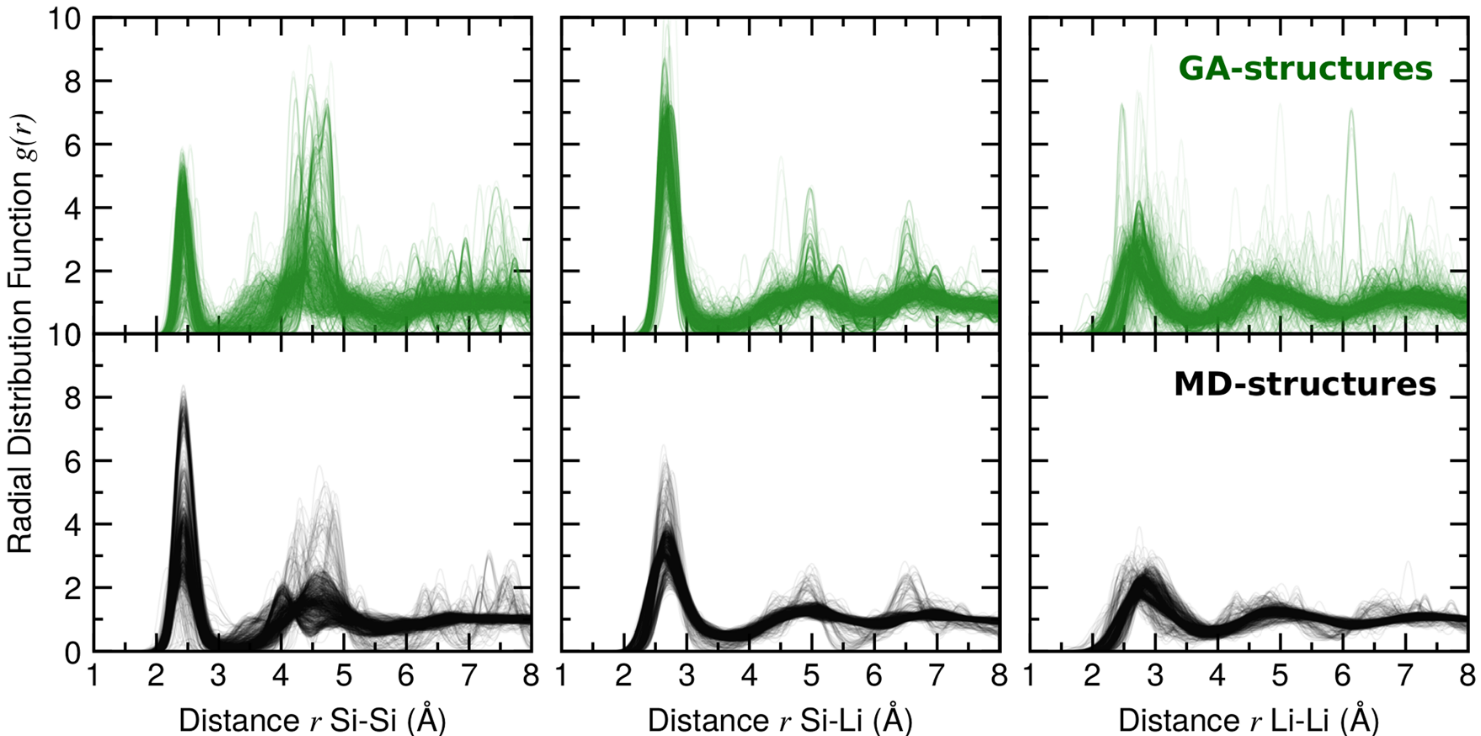
\includegraphics[width=\columnwidth]{LiSi-rdfs.png}
            \end{center}
            \tiny{Artrith \textit{et al.} (2018). \textit{The Journal of chemical
            physics}}

            \column{0.3\textwidth}
            \begin{itemize}
                \item Orden de largo alcance en GA. 
            \end{itemize}
        \end{columns}
            
    \end{frame}
    
    \begin{frame}
        \frametitle{Aplicaciones en baterías de litio: Li$_x$Si}
        
        \textbf{Simulaciones de dinámica molecular}

        \begin{columns}
            \column{0.6\textwidth}
            \begin{center}
                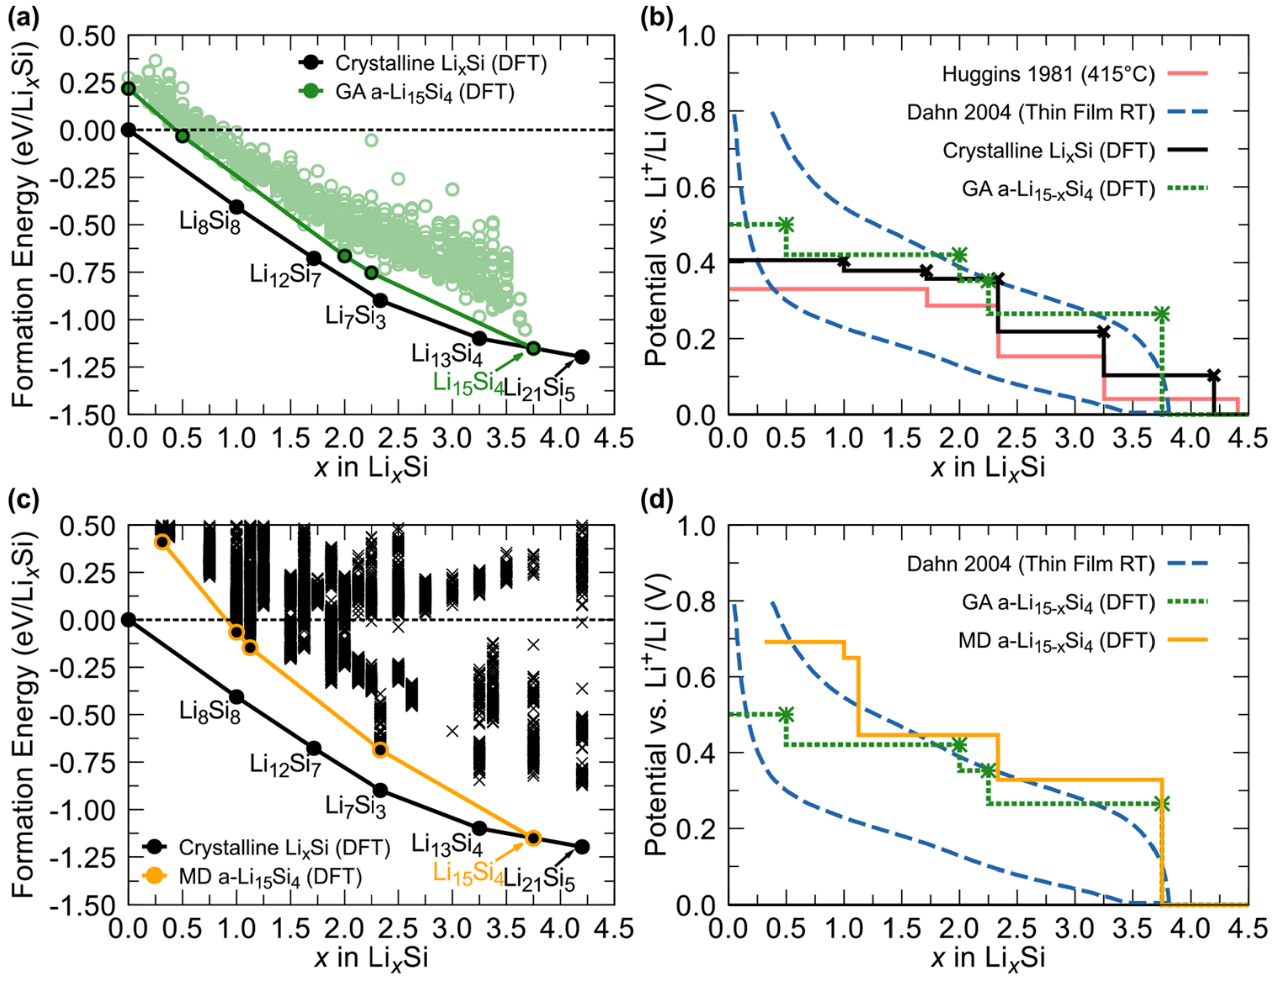
\includegraphics[width=\columnwidth]{LiSi-potencial_vs_Li.png}
            \end{center}
            
            \column{0.4\textwidth}
            \tiny{Artrith \textit{et al.} (2018). \textit{The Journal of chemical
            physics}}
        \end{columns}
            
    \end{frame}
    
    %%%% CONCLUSIONES %%%%
    \section{Conclusiones}

    \begin{frame}
        \frametitle{Conclusiones}

        Se pueden obtener potenciales interatómicos ajustando directamente la
        PES obtenida mediante cálculos de la estructura electrónica.
        
        \ \pause

        Los potenciales de aprendizaje automático están emergiendo como una nueva
        herramienta complementaria para el modelado de materiales y rápidamente 
        se están convirtiendo lo suficientemente flexibles para ser aplicados 
        en problemas reales de las ciencias de los materiales.


        \ \pause

        \textbf{Ventajas y desventajas de los potenciales de ML}:

        \pause 

        \begin{columns}
            \column{0.5\textwidth}
            \begin{itemize}
                \item Cómputo rápido a la hora de producción.
                \item Energías precisas, cercanas a las de los métodos de 
                    estructura electrónica (errores del orden de unos pocos 
                    meV/átomo).
            \end{itemize}

            \pause

            \column{0.5\textwidth}
            \begin{itemize}
                \item Se necesitan muchos datos de entrenamiento y es costoso 
                    generarlos.
                \item Son uno o dos órdenes de magnitud más lentos que los 
                    potenciales empíricos.
                \item Transferibilidad limitada. 
            \end{itemize}
        \end{columns}

    \end{frame}

    %%%% REFERENCIAS %%%%

    \begin{frame}
        \frametitle{Bibliografía consultada}

        \tiny{
            Deringer, V. L. (2020). Modelling and understanding battery 
                materials with machine-learning-driven atomistic simulations.
                \textit{Journal of Physics: Energy}, 2(4), 041003.
            
            Deringer, V. L., Caro, M. A., \& Csányi, G. (2019). Machine 
                learning interatomic potentials as emerging tools for materials 
                science. \textit{Advanced Materials}, 31(46), 1902765.

            Mishin, Y. (2021). Machine-learning interatomic potentials for 
                materials science. \textit{Acta Materialia}, 214, 116980.

            Behler, J. (2017). First principles neural network potentials 
                for reactive simulations of large molecular and condensed systems. 
                \textit{Angewandte Chemie International Edition}, 56(42), 12828-12840.

            Behler, J. (2016). Perspective: Machine learning potentials 
                for atomistic simulations. \textit{The Journal of chemical 
                physics}, 145(17), 170901.

            Mueller, T., Hernandez, A., \& Wang, C. (2020). Machine learning 
                for interatomic potential models. \textit{The Journal of chemical 
                physics}, 152(5), 050902.

            Hong, Y., Hou, B., Jiang, H., \& Zhang, J. (2020). Machine 
                learning and artificial neural network accelerated computational 
                discoveries in materials science. \textit{Wiley Interdisciplinary 
                Reviews: Computational Molecular Science}, 10(3), e1450.

            Botu, V., Batra, R., Chapman, J., \& Ramprasad, R. (2017). 
                Machine learning force fields: construction, validation, and 
                outlook. \textit{The Journal of Physical Chemistry C}, 121(1), 
                511-522.

            Li, W., Ando, Y., Minamitani, E., \& Watanabe, S. (2017). 
                Study of Li atom diffusion in amorphous Li3PO4 with neural 
                network potential. \textit{The Journal of chemical physics}, 
                147(21), 214106.

            Fujikake, S., Deringer, V. L., Lee, T. H., Krynski, M., 
                Elliott, S. R., \& Csányi, G. (2018). Gaussian approximation 
                potential modeling of lithium intercalation in carbon 
                nanostructures. \textit{The Journal of chemical physics}, 148(24), 241714.

            Artrith, N., Urban, A., \& Ceder, G. (2018). Constructing 
                first-principles phase diagrams of amorphous Li x Si using 
                machine-learning-assisted sampling with an evolutionary algorithm. 
                \textit{The Journal of chemical physics}, 148(24), 241711.
        }

    \end{frame}
    
    %%%% PREGUNTAS %%%%
    
    \begin{frame}
        \begin{center}
            \huge{¿Preguntas?}
        \end{center}
    \end{frame}

\end{document}
